\documentclass[12pt, a4paper]{report}

% --- PAQUETES DE IDIOMA Y CODIFICACIÓN ---
\usepackage[utf8]{inputenc}
\usepackage[T1]{fontenc}
\usepackage[spanish,es-tabla]{babel}

% --- TIPOGRAFÍA Y FORMATO DE PÁRRAFO ---
\usepackage{helvet}
\renewcommand{\familydefault}{\sfdefault}
\usepackage{parskip}
\setlength{\parskip}{10pt}
\usepackage{setspace}
\singlespacing
\usepackage[left=3cm,right=3cm,top=2.5cm,bottom=2.5cm]{geometry}

% --- COLORES Y GRÁFICOS ---
\usepackage{xcolor}
\definecolor{orcidlogocol}{HTML}{A6CE39}
\definecolor{mdpiBlue}{HTML}{2B7CB6}
\usepackage{tikz}
\usetikzlibrary{shapes.geometric, arrows.meta, positioning, fit, backgrounds, calc, decorations.pathreplacing, babel}
\usepackage{graphicx}
\graphicspath{{./images/}}

% --- TABLAS ---
\usepackage{booktabs}
\usepackage{caption}
\usepackage{longtable}
\usepackage{array}
\usepackage{tabularx}
\usepackage{multirow}
\usepackage{float}
\usepackage{pdflscape}

% --- MATEMÁTICAS Y SÍMBOLOS ---
\usepackage{amsmath, amssymb}
\usepackage{fontawesome5}

% --- BIBLIOGRAFÍA ---
\usepackage{csquotes}
\usepackage[style=authoryear, backend=biber]{biblatex}
\addbibresource{referencias.bib}

% --- TÍTULOS Y ESTRUCTURA ---
\usepackage{titlesec}
\usepackage{fancyhdr}
\usepackage{enumitem}

% Configuración para Figuras ---
\captionsetup[figure]{
    font={small},
    justification=centering,
    labelsep=period,
    skip=10pt
}

% --- CONFIGURACIÓN DE TÍTULOS ---
% Nivel 1: CAPÍTULOS
\titleformat{\chapter}[block]
  {\normalfont\fontsize{14}{16}\bfseries\filright}
  {\thechapter.}{1em}{}
\titlespacing*{\chapter}{0pt}{0pt}{10pt}

% Nivel 2: Sección
\titleformat{\section}
  {\normalfont\fontsize{14}{16}\bfseries\filright}
  {\thesection}{1em}{}

% Nivel 3: Subsección
\titleformat{\subsection}
  {\normalfont\fontsize{12}{14}\bfseries\filright}
  {\thesubsection}{1em}{}

% Nivel 4: Subsubsección
\titleformat{\subsubsection}
  {\normalfont\fontsize{12}{14}\bfseries\filright}
  {\thesubsubsection}{1em}{}

% Nivel 5: Párrafo
\titleformat{\paragraph}
  {\normalfont\fontsize{12}{14}\bfseries\filright}
  {\theparagraph}{1em}{}
\setcounter{secnumdepth}{5}

% Nivel 6: Subpárrafo
\titleformat{\subparagraph}[block]
  {\normalfont\fontsize{12}{14}\bfseries\filright}
  {\thesubparagraph}{1em}{\underline}

% --- ENLACES Y URLS ---
\usepackage{url}
\def\UrlBreaks{\do\/\do-\do_}
\usepackage{hyperref}
\hypersetup{
    colorlinks=true,
    citecolor=mdpiBlue,
    linkcolor=black,
    urlcolor=mdpiBlue
}

\emergencystretch=3em
\hbadness=10000
\hfuzz=50pt

% --- ENCABEZADOS Y NUMERACIÓN (Superior Derecha) ---
\pagestyle{fancy}
\fancyhf{}
\fancyhead[R]{\thepage}
\renewcommand{\headrulewidth}{0pt}
\setlength{\headheight}{14.5pt}

% --- CONFIGURACIÓN DE TABLAS Y FIGURAS (APA 7) ---
\captionsetup{labelsep=newline, justification=raggedright, singlelinecheck=false, font={small,bf}}

% --- QUITA EL SALTO DE PÁGINA ANTES DE CAPÍTULO ---
\usepackage{etoolbox}
\makeatletter
\patchcmd{\chapter}{\if@openright\cleardoublepage\else\clearpage\fi}{}{}{}
\makeatother

% Redefinir estilo plain para que sea igual al fancy
\fancypagestyle{plain}{
    \fancyhf{}
    \fancyhead[R]{\thepage}
    \renewcommand{\headrulewidth}{0pt}
}

% --- COMANDO PARA AUTORES CON ORCID ---
\newcommand{\autorconorcid}[3]{%
  \textbf{#1}, #2\quad%
  \href{https://orcid.org/#3}{\textcolor{orcidlogocol}{\faOrcid\ \underline{#3}}}%
}
\newcommand{\autorsinorcid}[2]{%
  \textbf{#1}, #2%
}

% ===================================================================
\begin{document}
% ===================================================================

% --- PORTADA ---
\begin{titlepage}
    \pagenumbering{gobble}
    \centering

    % Logo institucional UNJBG
    \begin{tikzpicture}
        % Escudo circular estilizado UNJBG
        \draw[line width=3pt, color=mdpiBlue] (0,0) circle (1.5cm);
        \draw[line width=1.5pt, color=mdpiBlue] (0,0) circle (1.1cm);
        \node[align=center, text=mdpiBlue, font=\bfseries\scriptsize] at (0, 0.55) {U N J B G};
        \node[align=center, text=mdpiBlue, font=\tiny] at (0, 0.1) {TACNA -- PERÚ};
        \draw[color=mdpiBlue, line width=1pt] (-0.7,-0.25) -- (0.7,-0.25);
        \node[align=center, text=mdpiBlue, font=\bfseries\large] at (0, -0.7) {\faUniversity};
        \draw[color=mdpiBlue!60, line width=0.5pt] (0,0) circle (1.3cm);
    \end{tikzpicture}
    \par\vspace{0.2cm}
    {\fontsize{13}{15}\bfseries\color{mdpiBlue} Universidad Nacional Jorge Basadre Grohmann\par}
    {\fontsize{12}{14}\selectfont Escuela Profesional de Ingeniería en Informática y Sistemas\par}

    \vspace{0.6cm}
    {\fontsize{14}{16}\bfseries REDES I\par}
    {\fontsize{12}{14}\bfseries MEMORIA TÉCNICA\par}
    \vspace{0.2cm}
    {\fontsize{12}{14}\bfseries Diseño de la Infraestructura Física y Cableado Estructurado\\
    de una Red LAN — Policlínico de Especialidades Médicas\\
    ``Salud \& Vida'' S.A.C.\par}

    \vspace{0.5cm}

    \begin{center}
        {\bfseries Docente:}\\[0.2cm]
        \normalsize Mg. REYNALDO ALFONTE ZAPANA
    \end{center}

    \vspace{0.4cm}

    \begin{flushleft}
        {\bfseries Autores:}\\[0.4cm]
        \small
        \autorconorcid{Cachicatari Quito Aron Rene}{2024-119011}{0009-0001-0343-6817}\\[0.3cm]
        \autorsinorcid{Banchello Pino Rojas Raul Farid}{2024-119009}\\[0.3cm]
        \autorconorcid{Nina Estuco William Andre}{2024-119006}{0009-0002-6296-4473}\\[0.3cm]
        \autorsinorcid{Mamani Lima Josue Fernando}{2025-19055}\\[0.3cm]
        \autorconorcid{Briceño Pihuaycho Fernando Jesus}{2024-119029}{0009-0004-2188-6274}\\[0.3cm]
    \end{flushleft}

    \vspace{0.3cm}

    \begin{center}
        \begin{minipage}{0.96\textwidth}
            {\small \textbf{RESUMEN:} La presente memoria técnica documenta el diseño completo de la infraestructura de red LAN del Policlínico de Especialidades Médicas ``Salud \& Vida'' S.A.C., una edificación de 450~m$^2$ de planta única. El estudio cubre la definición de requerimientos (48~tomas activas + 8~de reserva = 56~puertos totales), la selección de topología física en estrella jerárquica con medios UTP~Cat~6 LSZH y F/UTP~Cat~6A blindado, la ingeniería de cableado estructurado bajo normas ANSI/TIA-568, 569, 606 y 607, el diseño físico del rack 42U con el cuadro de materiales valorizado en USD~\$9,632 y el protocolo de construcción y certificación del cableado bajo el estándar T568B, con distancia máxima de enlace permanente de 34.8~m, en un amplio margen sobre el límite normativo de 90~m.\par}

            \vspace{0.2cm}
            {\small \textbf{Palabras clave:} Cableado estructurado, ANSI/TIA-568, Red LAN hospitalaria, Cat~6 LSZH, F/UTP Cat~6A, Rack 42U, UPS, Wi-Fi~6, Certificación de enlace.\par}

            \vspace{0.3cm}
            {\small \textbf{ABSTRACT:} This technical report documents the complete LAN network infrastructure design for the ``Salud \& Vida'' Medical Specialty Polyclinic, a single-floor 450~m$^2$ building. The study covers requirements definition (48 active outlets + 8 spare = 56 total ports), hierarchical star topology selection with UTP~Cat~6 LSZH and shielded F/UTP~Cat~6A media, structured cabling engineering under ANSI/TIA-568, 569, 606 and 607 standards, a 42U rack physical design with a material list valued at USD~\$9,632, and the cable construction and certification protocol under the T568B standard, with a maximum permanent link distance of 34.8~m — well within the 90~m normative limit.\par}

            \vspace{0.2cm}
            {\small \textbf{Keywords:} Structured cabling, ANSI/TIA-568, Hospital LAN, Cat~6 LSZH, F/UTP~Cat~6A, 42U rack, UPS, Wi-Fi~6, Link certification.\par}
        \end{minipage}
    \end{center}

    \vfill
    {\normalsize Tacna, Octubre 2026\par}
\end{titlepage}


\newpage
\pagenumbering{roman}
\setcounter{page}{1}
\tableofcontents

\newpage
% --- INICIO DEL CUERPO ---
\pagenumbering{arabic}
\setcounter{page}{1}

% --- CAPÍTULOS ---
\chapter*{INTRODUCCIÓN}
\addcontentsline{toc}{chapter}{INTRODUCCIÓN}

El acceso oportuno a la información clínica es un pilar fundamental de la atención médica moderna. Un sistema de red local bien diseñado permite que los historiales clínicos electrónicos, imágenes radiológicas DICOM y registros de farmacia fluyan de forma inmediata entre los profesionales de salud, reduciendo tiempos de diagnóstico y minimizando errores derivados del uso de documentación en papel.

La presente memoria técnica documenta de manera exhaustiva y sistematizada el proyecto de diseño de la infraestructura física de red LAN del \textbf{Policlínico de Especialidades Médicas ``Salud \& Vida'' S.A.C.}, una edificación de \textbf{450~m$^2$ de planta única} ubicada en la ciudad de Tacna. El proyecto ha sido desarrollado como trabajo integrador de la asignatura \textbf{Redes I (Unidad I: Infraestructura de Red)}, cubriendo desde la definición de requerimientos organizacionales hasta el protocolo de certificación y la confección manual de la muestra física de cableado.

\section*{Objetivo General}

Diseñar la infraestructura de red de área local (LAN) del Policlínico ``Salud \& Vida'' S.A.C., bajo los estándares internacionales ANSI/TIA, garantizando conectividad Gigabit a todos los puestos de trabajo y disponibilidad de red inalámbrica Wi-Fi~6 en toda la planta, dentro de un presupuesto optimizado y con los márgenes técnicos requeridos para una operación de misión crítica médica.

\section*{Objetivos Específicos}

\begin{enumerate}[leftmargin=*, label=\arabic*.]
    \item Identificar y clasificar todos los ambientes, dispositivos y requerimientos de conectividad de la organización.
    \item Seleccionar y justificar la topología de red, los modelos de referencia y los medios de transmisión más apropiados para el entorno hospitalario.
    \item Diseñar el sistema de cableado estructurado bajo los estándares ANSI/TIA-568, 569, 606 y 607, incluyendo la distribución del gabinete rack 42U y el mapa de parcheo de los 56 puertos proyectados.
    \item Elaborar los planos físicos de distribución de tomas, canalizaciones y cobertura inalámbrica, junto con el cuadro de materiales valorizado (BOM).
    \item Definir el protocolo de construcción de cables UTP y el plan de pruebas de certificación, preparando al equipo para la defensa técnica individual ante el docente.
\end{enumerate}

\section*{Alcance y Limitaciones}

El alcance del proyecto comprende únicamente la \textbf{Unidad I: Infraestructura Física y Cableado Estructurado}. El direccionamiento IP, enrutamiento, seguridad lógica y servicios de red (DHCP, DNS, VPN) corresponden a unidades posteriores de la asignatura y quedan explícitamente fuera del alcance del presente documento.

\section*{Estructura del Documento}

La memoria se organiza en cinco capítulos, que corresponden a las cinco etapas del proyecto:

\begin{itemize}[leftmargin=*]
    \item \textbf{Capítulo 1:} Definición de la organización, inventario de ambientes y matriz de requerimientos de red.
    \item \textbf{Capítulo 2:} Selección de topología, aplicación de los modelos OSI/TCP-IP y justificación de los medios de transmisión.
    \item \textbf{Capítulo 3:} Ingeniería de cableado estructurado, diseño del rack 42U y cómputo de materiales.
    \item \textbf{Capítulo 4:} Planos de distribución física, diseño de canalizaciones, cobertura Wi-Fi~6 y BOM valorizado.
    \item \textbf{Capítulo 5:} Construcción de cable UTP bajo norma T568B y plan de pruebas de certificación.
\end{itemize}

\chapter{Definición de la Organización y Requerimientos de Red}

\section{Descripción de la Organización}

El \textbf{Policlínico de Especialidades Médicas ``Salud \& Vida'' S.A.C.} es una institución de salud privada de nivel ambulatorio que brinda atención multidisciplinaria especializada. Se ubica en Tacna, Perú, y opera en una infraestructura de \textbf{planta única de 450~m$^2$ (30.00~m $\times$ 15.00~m)}.

\subsection{Misión y Perfil Tecnológico}

La organización requiere una red de datos de alta disponibilidad para soportar la gestión digital de historiales clínicos electrónicos (EMR/HCE), la transferencia de imágenes radiológicas en estándar DICOM, el control de inventarios de farmacia y la comunicación interna mediante telefonía IP (VoIP).

\begin{figure}[H]
\centering
\begin{tikzpicture}[
    scale=0.92, transform shape,
    box/.style={draw, rounded corners=3pt, fill=mdpiBlue!12, minimum width=2.8cm, minimum height=0.7cm, align=center, font=\footnotesize\bfseries, text=mdpiBlue!90!black},
    jefe/.style={draw, rounded corners=3pt, fill=mdpiBlue, minimum width=3.8cm, minimum height=0.75cm, align=center, font=\small\bfseries, text=white},
    linea/.style={-Stealth, thick, color=mdpiBlue!70}
]
\node[jefe] (dir) at (0,0) {Dirección General};
\node[box] (adm) at (-4.2,-1.6) {Administración\\Jefatura};
\node[box] (med) at (0,-1.6) {Área Médica\\(8 consultorios)};
\node[box] (diag) at (4.2,-1.6) {Diagnóstico\\Rayos~X / Lab.};
\node[box] (rec) at (-3.5,-3.3) {Recepción\\y Caja};
\node[box] (farm) at (0,-3.3) {Farmacia\\Asistencial};
\node[box] (triaje) at (3.5,-3.3) {Triaje\\y Tópico};
\draw[linea] (dir) -- (adm);
\draw[linea] (dir) -- (med);
\draw[linea] (dir) -- (diag);
\draw[linea] (adm) -- (rec);
\draw[linea] (med) -- (farm);
\draw[linea] (med) -- (triaje);
\end{tikzpicture}
\caption{Organigrama funcional del Policlínico ``Salud \& Vida'' S.A.C.}
\label{fig:organigrama}
\end{figure}

\subsection{Número de Trabajadores y Dispositivos}

La plantilla operativa asciende a \textbf{38 a 50 personas} entre médicos, enfermeras, técnicos, personal administrativo y personal de apoyo. El número de dispositivos de red que operan simultáneamente varía entre \textbf{44 y 50 terminales activos}, dentro del rango exigido por la rúbrica del proyecto (30 a 60 dispositivos).

\section{Inventario de Ambientes y Distribución de Planta}

La edificación se organiza en tres zonas funcionales claramente diferenciadas, tal como se muestra en el plano arquitectónico interactivo diseñado en SVG a escala 1:100:

\subsection{Zona Norte: Consultorios y Servicios Médicos}

\begin{table}[H]
\centering
\caption{Inventario de ambientes — Ala Norte}
\begin{tabularx}{\textwidth}{@{} >{\raggedright\arraybackslash}p{5.5cm} c c X @{}}
\toprule
\textbf{Ambiente} & \textbf{Dimensiones} & \textbf{Área} & \textbf{Función Principal} \\
\midrule
MDF (Telecomunicaciones) & 3.50~m $\times$ 4.20~m & 14.7~m$^2$ & Cuarto central de comunicaciones \\
Recepción / Admisión / Caja & 6.00~m $\times$ 4.20~m & 25.2~m$^2$ & Atención al público y facturación \\
Consultorio 01 & 3.50~m $\times$ 4.20~m & 14.7~m$^2$ & Medicina General \\
Consultorio 02 & 3.50~m $\times$ 4.20~m & 14.7~m$^2$ & Pediatría \\
Consultorio 03 & 3.50~m $\times$ 4.20~m & 14.7~m$^2$ & Ginecología \\
Consultorio 04 & 3.50~m $\times$ 4.20~m & 14.7~m$^2$ & Cardiología \\
Consultorio 05 & 3.50~m $\times$ 4.20~m & 14.7~m$^2$ & Traumatología \\
Farmacia Asistencial & 3.50~m $\times$ 4.20~m & 14.7~m$^2$ & Dispensación de medicamentos \\
\bottomrule
\end{tabularx}
\label{tab:ambientes-norte}
\end{table}

\subsection{Zona Central: Pasillo y Circulación}

El pasillo central de \textbf{30.00~m $\times$ 2.40~m (72~m$^2$)} constituye el eje troncal del sistema de canalización. Aloja la bandeja portacables tipo malla de 200$\times$50~mm suspendida a 2.75~m de altura, y los puntos de acceso Wi-Fi~6 AP-02 y AP-03 anclados al cielo raso.

\subsection{Zona Sur: Diagnóstico, Especialidades y Administración}

\begin{table}[H]
\centering
\caption{Inventario de ambientes — Ala Sur}
\begin{tabularx}{\textwidth}{@{} >{\raggedright\arraybackslash}p{5.5cm} c c X @{}}
\toprule
\textbf{Ambiente} & \textbf{Dimensiones} & \textbf{Área} & \textbf{Función Principal} \\
\midrule
Sala de Espera General & 7.00~m $\times$ 7.00~m & 49.0~m$^2$ & Sala pública para 35 personas \\
Triaje y Tópico & 3.50~m $\times$ 4.20~m & 14.7~m$^2$ & Registro y urgencias \\
Consultorio 06 & 3.50~m $\times$ 4.20~m & 14.7~m$^2$ & Oftalmología \\
Consultorio 07 & 3.50~m $\times$ 4.20~m & 14.7~m$^2$ & Odontología \\
Consultorio 08 & 3.50~m $\times$ 4.20~m & 14.7~m$^2$ & Psicología / Nutrición \\
Laboratorio Clínico & 4.50~m $\times$ 4.20~m & 18.9~m$^2$ & Bioquímica y análisis clínicos \\
Diagnóstico por Imágenes (Rayos~X) & 5.00~m $\times$ 4.20~m & 21.0~m$^2$ & Radiología y ecografía \\
Administración / Jefatura & 3.50~m $\times$ 7.00~m & 24.5~m$^2$ & Gestión administrativa y contable \\
\bottomrule
\end{tabularx}
\label{tab:ambientes-sur}
\end{table}

\section{Justificación de la Ubicación Geocéntrica del MDF}

El \textbf{Cuarto de Telecomunicaciones (MDF)} se sitúa en la posición central del edificio, con coordenadas georreferenciadas en el plano SVG de \(X = 14.00~\text{m},\; Y = 2.10~\text{m}\). Esta decisión reduce la distancia de la tirada horizontal más larga a \textbf{34.80~m} (Laboratorio Clínico), lo que representa apenas el \textbf{38.7\% del límite máximo de 90~m} establecido por la norma ANSI/TIA-568, otorgando un margen de seguridad superior al 61\%.

\section{Marco de Requerimientos de Red (Sección 6)}

\subsection{Cobertura de Red Inalámbrica (WLAN Wi-Fi 6)}

Se proyectan \textbf{cuatro Puntos de Acceso (APs) Wi-Fi~6 (IEEE~802.11ax)} PoE+ con radio efectivo de 8.0~m en banda de 5~GHz, distribuidos estratégicamente:

\begin{itemize}[leftmargin=*]
    \item \textbf{AP-01:} Sala de Espera General — red pública de cortesía para pacientes y pantalla de turnos.
    \item \textbf{AP-02:} Pasillo Central Oeste — cobertura médica a Consultorios 1 al 4 y Triaje.
    \item \textbf{AP-03:} Pasillo Central Este — cobertura médica a Consultorios 5 al 8 y Laboratorio.
    \item \textbf{AP-04:} Administración General (sector este) — cobertura corporativa a jefatura y contabilidad.
\end{itemize}

\subsection{Matriz de Requerimientos de Red por Ambiente}

\begin{table}[H]
\centering
\caption{Matriz de requerimientos de red por ambiente}
\small
\begin{tabularx}{\textwidth}{@{} c >{\raggedright\arraybackslash}p{4.2cm} X c >{\centering\arraybackslash}p{2.4cm} @{}}
\toprule
\textbf{N°} & \textbf{Ambiente} & \textbf{Dispositivos Asignados} & \textbf{Tomas} & \textbf{Medio Físico} \\
\midrule
1  & Admisión, Caja y Recepción & 3 PCs, 1 impresora, 2 VoIP & 6 & UTP Cat~6 \\
2  & Sala de Espera General    & 1 Smart TV, 1 AP-01 PoE & 2 & UTP Cat~6 \\
3  & Triaje y Tópico           & 2 PCs, 1 teléfono IP & 3 & UTP Cat~6 \\
4--8 & Consultorios 1 al 5     & 5 PCs, 5 teléfonos IP & 10 & UTP Cat~6 \\
9--11 & Consultorios 6 al 8   & 3 PCs, 3 teléfonos IP & 6 & UTP Cat~6 \\
12 & Laboratorio Clínico       & 2 PCs, 1 analizador bioquímico & 3 & F/UTP Cat~6A \\
13 & Rayos~X y Ecografía       & 2 estaciones DICOM, 1 impresora & 3 & F/UTP Cat~6A \\
14 & Farmacia Asistencial      & 2 terminales venta, 1 imp. térmica & 3 & UTP Cat~6 \\
15 & Administración y Jefatura & 4 PCs, 1 multifuncional, 1 VoIP, 1 AP & 7 & UTP Cat~6 \\
16 & Pasillo Central (APs)     & AP-02, AP-03 PoE Wi-Fi~6 & 2 & UTP Cat~6 \\
17 & MDF (Servidores)          & Servidor HCE, Servidor PACS, NAS & 3 & F/UTP Cat~6A \\
\midrule
   & \textbf{Subtotal Activos}  &  & \textbf{48} & \\
   & Reserva técnica ($>$15\%) &  & \textbf{8}  & \\
\midrule
   & \textbf{TOTAL PARCHEO}     &  & \textbf{56} & \\
\bottomrule
\end{tabularx}
\label{tab:requerimientos-red}
\end{table}

\subsection{Resumen de Características Técnicas Identificadas}

\begin{itemize}[leftmargin=*]
    \item \textbf{Rango de dispositivos simultáneos:} 44 a 50 terminales activos (dentro del rango de 30 a 60 exigido).
    \item \textbf{Tráfico crítico de imágenes médicas:} Archivos DICOM de 50~MB a 300~MB por estudio radiológico.
    \item \textbf{Tráfico VoIP:} Sensible a latencia y jitter; requiere calidad de servicio (QoS).
    \item \textbf{Zonas con EMI elevada:} Rayos~X (tubo de 100~kV) y Laboratorio (centrífugas y analizadores) exigen cable blindado F/UTP Cat~6A y puesta a tierra bajo ANSI/TIA-607-C.
    \item \textbf{Seguridad ante incendios:} Forro LSZH obligatorio en entornos hospitalarios (IEC~60332-1).
\end{itemize}

\chapter{Topología, Modelos de Referencia y Selección de Medios de Transmisión}

\section{Tipo y Clasificación de la Red}

\subsection{Clasificación por Alcance Geográfico}

La infraestructura proyectada se clasifica como una \textbf{Red de Área Local (LAN --- Local Area Network)} combinada con un segmento inalámbrico \textbf{WLAN (Wireless Local Area Network)}:

\begin{itemize}[leftmargin=*]
    \item \textbf{Cobertura espacial:} Confinada dentro del predio del policlínico: 30~m $\times$ 15~m (450~m$^2$, planta única).
    \item \textbf{Propiedad:} Red privada de administración interna exclusiva de la institución de salud.
    \item \textbf{Tasa de transferencia proyectada:} \textbf{1~Gbps} (1000BASE-T) en puestos de trabajo y \textbf{10~Gbps} (10GBASE-T) en el enlace troncal hacia servidores y el switch de distribución.
    \item \textbf{Componente WLAN (IEEE~802.11ax --- Wi-Fi~6):} Cuatro APs PoE+ con células de cobertura de \textbf{8.0~m de radio efectivo a 5~GHz}, con solapamiento controlado del 15\% para garantizar \textit{Fast Roaming} (802.11r/k/v) del personal médico en movimiento.
\end{itemize}

\section{Topología Física: Estrella Jerárquica}

Se ha seleccionado una \textbf{Topología Física en Estrella Jerárquica} con un único nodo central de consolidación en el \textbf{Cuarto de Telecomunicaciones (MDF --- Main Distribution Frame)}.

\subsection{Justificación Técnica de la Topología}

\begin{enumerate}[leftmargin=*, label=\arabic*.]
    \item \textbf{Aislamiento de fallas:} Si un jack o cable horizontal en un consultorio sufre daño físico, el fallo queda completamente aislado a ese puerto sin afectar a los demás ambientes.
    \item \textbf{Centralización del mantenimiento:} Toda la conmutación, parcheo, respaldo eléctrico (UPS) y monitoreo se concentran en el Rack~42U del MDF, facilitando la auditoría bajo ANSI/TIA-606-B.
    \item \textbf{Optimización de recorridos:} Al situar el MDF en el centro geográfico del edificio, la longitud máxima de cable horizontal hasta la toma más lejana es de \textbf{34.8~m}, muy por debajo del límite de \textbf{90~m} de la norma ANSI/TIA-568.
    \item \textbf{Escalabilidad:} La incorporación de nuevos puntos de red solo requiere tender un cable adicional desde el puesto de trabajo hasta el patch panel, sin reestructurar el tendido existente.
\end{enumerate}

\begin{figure}[H]
\centering
\begin{tikzpicture}[
    ap/.style={circle, draw, fill=orange!20, minimum size=0.9cm, font=\tiny\bfseries},
    pc/.style={rectangle, draw, fill=gray!15, minimum width=1.1cm, minimum height=0.55cm, rounded corners=2pt, font=\tiny},
    sw/.style={rectangle, draw, fill=mdpiBlue, text=white, minimum width=2.2cm, minimum height=0.7cm, font=\small\bfseries},
    rack/.style={rectangle, draw, fill=mdpiBlue!80, text=white, minimum width=2.6cm, minimum height=0.9cm, rounded corners=3pt, font=\small\bfseries},
    link/.style={thick, color=mdpiBlue!60},
    wlink/.style={dashed, thick, color=orange!70}
]
% MDF central
\node[rack] (mdf) at (0,0) {MDF Rack 42U};
% Switches
\node[sw] (sw1) at (-3.5, 0) {SW Acceso 01};
\node[sw] (sw2) at (3.5, 0) {SW Acceso 02};
\draw[link, double] (mdf) -- (sw1) node[midway, above, font=\tiny] {10G};
\draw[link, double] (mdf) -- (sw2) node[midway, above, font=\tiny] {10G};
% Nodos ala norte
\node[pc] (c1) at (-6.5,  1.4) {C01 Med.Gral};
\node[pc] (c2) at (-6.5,  0.5) {C02 Ped.};
\node[pc] (c3) at (-6.5, -0.4) {C03 Gin.};
\node[pc] (rec) at (-6.5,-1.3) {Recepción};
\node[pc] (far) at (-6.5,-2.2) {Farmacia};
\foreach \n in {c1,c2,c3,rec,far} \draw[link] (sw1) -- (\n);
% Nodos ala sur
\node[pc] (c6) at (6.5,  1.4) {C06 Oftal.};
\node[pc] (c7) at (6.5,  0.5) {C07 Odont.};
\node[pc] (lab) at (6.5, -0.4) {Laboratorio};
\node[pc] (rx)  at (6.5, -1.3) {Rayos~X};
\node[pc] (adm) at (6.5, -2.2) {Adm.};
\foreach \n in {c6,c7,lab,rx,adm} \draw[link] (sw2) -- (\n);
% APs
\node[ap] (ap1) at (-1.5, 2.4) {AP-01};
\node[ap] (ap2) at (-0.5, 2.4) {AP-02};
\node[ap] (ap3) at (0.5, 2.4)  {AP-03};
\node[ap] (ap4) at (1.5, 2.4)  {AP-04};
\draw[wlink] (mdf) -- (ap1);
\draw[wlink] (mdf) -- (ap2);
\draw[wlink] (mdf) -- (ap3);
\draw[wlink] (mdf) -- (ap4);
\end{tikzpicture}
\caption{Diagrama de topología física en estrella jerárquica del Policlínico ``Salud \& Vida''. Las líneas continuas representan cableado UTP/F-UTP y las líneas punteadas los enlaces PoE+ a los APs Wi-Fi~6.}
\label{fig:topologia}
\end{figure}

\subsection{Topología Lógica: Punto a Punto Conmutado}

La topología lógica opera mediante \textbf{enlaces punto a punto Full-Duplex conmutados (Switched Ethernet --- IEEE~802.3ab)}. Cada estación dispone de un canal exclusivo de \textbf{1~Gbps simétrico} hacia el puerto del switch, eliminando completamente los dominios de colisión que existían en redes antiguas de tipo bus.

\section{Aplicación de los Modelos de Referencia OSI y TCP/IP}

\subsection{Correspondencia de Capas Aplicada al Policlínico}

\begin{table}[H]
\caption{Correspondencia de capas OSI / TCP-IP con componentes del policlínico}
\begin{tabularx}{\textwidth}{@{}ccXX@{}}
\toprule
\textbf{OSI} & \textbf{TCP/IP} & \textbf{Componente Real} & \textbf{Función en la Infraestructura} \\
\midrule
7. Aplicación & Aplicación & Software EMR, visor DICOM, navegador de facturación & Interfaz de software médico con la que interactúan los usuarios \\
6. Presentación & Aplicación & Formatos DICOM, HL7, cifrado SSL/TLS & Estandarización y cifrado de datos clínicos sensibles \\
5. Sesión & Aplicación & Keep-Alive, RPC entre PC médica y servidor HCE & Mantiene la sesión de atención sin pérdida de datos \\
4. Transporte & Transporte & TCP (HCE, recetas) / UDP (VoIP, turnero TV) & Segmentación y asignación de puertos de origen y destino \\
3. Red & Internet & Direccionamiento IPv4 (\textit{configurado en Unidad~II}) & Identificación lógica de nodos y servidores \\
2. Enlace & Acceso Red & NICs con direcciones MAC, switches Layer~2, tramas Ethernet (IEEE~802.3) & Detección de errores CRC-32 y control de acceso al medio \\
\textbf{1. Física} & \textbf{Acceso Red} & \textbf{Cable UTP Cat~6, F/UTP Cat~6A, jacks RJ-45, patch panels, señales Wi-Fi~6} & \textbf{Conversión de bits en señales eléctricas en los pares de cobre} \\
\bottomrule
\end{tabularx}
\label{tab:capas-osi}
\end{table}

\subsection{Ejemplo de Encapsulación: Envío de Estudio Radiológico al Servidor PACS}

Cuando el tecnólogo médico en la sala de Rayos~X envía una imagen radiológica al servidor PACS del rack, el proceso de encapsulación recorre las capas del modelo en orden descendente:

\begin{enumerate}[leftmargin=*, label=\arabic*.]
    \item \textbf{Capa 7/6/5:} El estudio DICOM (50--300~MB) se genera con metadatos clínicos y matriz de píxeles.
    \item \textbf{Capa 4 (TCP):} El archivo se divide en segmentos de \textbf{MSS = 1460~bytes} con puerto de destino \textbf{TCP/104} (estándar DICOM Storage).
    \item \textbf{Capa 3 (IP):} Se añaden cabeceras IP de origen (PC Rayos~X) y destino (Servidor PACS).
    \item \textbf{Capa 2 (Ethernet):} Se encierra en tramas Ethernet con cabecera MAC y cola \textbf{FCS CRC-32} para detección de errores.
    \item \textbf{Capa 1 (Física):} Los bits se codifican en niveles de tensión mediante modulación \textbf{4D-PAM5} y se transmiten en paralelo por los cuatro pares del cable F/UTP Cat~6A apantallado.
\end{enumerate}

\section{Sistemas y Medios de Comunicación}

\subsection{Señales y Esquema de Codificación}

El estándar \textbf{1000BASE-T (Gigabit Ethernet)} emplea los cuatro pares de cobre simultáneamente en modo full-duplex bidireccional con modulación \textbf{4D-PAM5}:

\begin{equation}
\text{Tasa Total} = 125~\text{MBaudios} \times 2~\frac{\text{bits}}{\text{baudio}} \times 4~\text{pares} = \mathbf{1000~\text{Mbps}} = 1~\text{Gbps}
\end{equation}

\subsection{Capacidad del Canal: Teorema de Shannon-Hartley}

En zonas con alto ruido electromagnético como Rayos~X, si no se emplea blindaje físico, la relación señal a ruido (SNR) decae y la capacidad teórica del canal disminuye:

\begin{equation}
C = B \log_2 \!\left(1 + \frac{S}{N}\right)
\end{equation}

Esto justifica técnicamente el uso de cable \textbf{F/UTP Cat~6A apantallado} en las salas con equipos inductivos, cuya pantalla de aluminio logra una eficacia de aislamiento electromagnético $\geq 40~\text{dB}$ en el rango de 30~MHz a 1000~MHz.

\section{Selección y Justificación de Medios de Transmisión}

\subsection{Matriz Comparativa de Medios Físicos}

\begin{table}[H]
\caption{Matriz comparativa de medios de transmisión}
\begin{tabularx}{\textwidth}{@{}Xccccc@{}}
\toprule
\textbf{Criterio} & \textbf{UTP Cat~6} & \textbf{F/UTP Cat~6A} & \textbf{Coaxial} & \textbf{FO Multimodo} & \textbf{FO Monomodo} \\
\midrule
Ancho de Banda & 250~MHz & 500~MHz & $\leq$1~GHz & 4700~MHz·km & $\sim$THz \\
Velocidad LAN & 1~Gbps & 10~Gbps & $<$100~Mbps & 10--100~Gbps & $>$10~Gbps \\
Dist. Máxima & 90~m & 90~m & 185~m & 300--550~m & $>$10~km \\
Inmunidad EMI & Media & \textbf{Muy alta} & Media-Alta & \textbf{Total} & \textbf{Total} \\
Costo/metro & Bajo & Moderado & Obsoleto & Alto & Alto \\
Uso en Proyecto & \textbf{85\%} & \textbf{15\%} & Descartado & Uplink Rack & Descartado \\
\bottomrule
\end{tabularx}
\label{tab:medios}
\end{table}

\subsection{Decisiones de Selección Justificadas}

\subsubsection{Cable UTP Categoría 6 LSZH para el 85\% de las tomas}

Soporta holgadamente \textbf{1~Gbps a 250~MHz} para todas las aplicaciones médico-administrativas. El forro \textbf{LSZH (Low Smoke Zero Halogen)} es obligatorio en centros de salud: en caso de incendio no propaga la llama ni emite gases halógenos tóxicos, protegiendo a pacientes de movilidad reducida.

\subsubsection{Cable F/UTP Categoría 6A Apantallado para Rayos X y Laboratorio}

La pantalla de aluminio aisla los picos electromagnéticos del tubo de Rayos~X (100~kV), evitando la corrupción de las tramas DICOM durante la transferencia al servidor PACS. La categoría 6A (500~MHz, 10~Gbps) soporta los archivos de 50--300~MB sin degradación de velocidad.

\subsubsection{Descarte del Cable Coaxial}

El cable coaxial (10BASE2 / 10BASE5) es una tecnología obsoleta desde la década de 1990. Su topología en bus compartido introduce colisiones masivas, no soporta conmutación full-duplex y sus conectores BNC son incompatibles con los switches modernos de Gigabit Ethernet.

\subsubsection{Fibra Óptica solo en el Troncal del Rack}

La fibra hasta el escritorio (\textit{FTTD}) es antieconómica para distancias cortas (menores a 40~m). En el MDF se usan cables DAC (\textit{Direct Attach Copper}) o latiguillos de fibra multimodo \textbf{OM3} para interconectar los switches y los servidores a \textbf{10~Gbps (10GBASE-SR)}, eliminando cuellos de botella en el núcleo de la red.

\chapter{Cableado Estructurado, Diseño del Rack 42U y Cómputo de Materiales}

\section{Marco Normativo Internacional Aplicable}

El diseño e implementación de la red física se rige bajo los estándares unificados de la \textbf{Telecommunications Industry Association (TIA)} y el \textbf{American National Standards Institute (ANSI)}:

\begin{enumerate}[leftmargin=*, label=\arabic*.]
    \item \textbf{ANSI/TIA-568.0-D y 568-C.2:} Establece la topología en estrella jerárquica y fija la distancia máxima del \textbf{Enlace Permanente} en \textbf{90~m}, con hasta 10~m para latiguillos, totalizando un Canal de máximo \textbf{100~m}.
    \item \textbf{ANSI/TIA-569-D:} Regula las dimensiones de canalizaciones. La ocupación inicial de cables en bandejas no debe exceder el \textbf{40\%} del área transversal, reservando el 50\% restante para crecimiento futuro.
    \item \textbf{ANSI/TIA-606-B:} Define el esquema alfanumérico para etiquetado unívoco de cables, tomas, paneles y gabinetes, garantizando la trazabilidad de cada enlace.
    \item \textbf{ANSI/TIA-607-C:} Prescribe la infraestructura de puesta a tierra equipotencial (bonding) para drenar corrientes de blindaje del cable F/UTP Cat~6A en Rayos~X y Laboratorio.
\end{enumerate}

\section{Subsistemas de Cableado Estructurado}

Al tratarse de una edificación de \textbf{un solo nivel}, no se requiere un subsistema de cableado troncal vertical entre pisos. La infraestructura se concentra en tres subsistemas operativos:

\subsection{Subsistema de Área de Trabajo (WA)}

Comprende desde la toma de pared (caja adosada con \textit{faceplate} y jacks RJ-45 Keystone hembra) hasta el equipo del usuario. Se utilizan \textbf{patch cords multifilares Cat~6 / Cat~6A de 2.0~m}, certificados de fábrica para resistir dobladuras diarias.

\subsection{Subsistema de Cableado Horizontal}

Transporta las señales desde las tomas de usuario hasta los patch panels del MDF. Emplea cable rígido monofilamento AWG~23 con forro ignífugo \textbf{LSZH}. No se permiten empalmes ni derivaciones intermedias: todos los enlaces son punto a punto directos.

\subsection{Subsistema del Cuarto de Telecomunicaciones (MDF)}

Espacio cerrado de \textbf{3.50~m $\times$ 4.20~m (14.7~m$^2$)} en el centro geográfico del edificio. Aloja el bastidor principal Rack~42U con patch panels, switches, servidores, UPS y el sistema de tierra de telecomunicaciones (TMGB).

\section{Diseño de Canalizaciones (ANSI/TIA-569-D)}

\subsection{Troncal Principal: Bandeja Tipo Malla en Pasillo Central}

\begin{itemize}[leftmargin=*]
    \item \textbf{Trayectoria:} Línea recta de 30~m suspendida a \textbf{2.75~m} en el plenum del cielo raso.
    \item \textbf{Dimensiones:} Ancho de \textbf{200~mm}, peralte de \textbf{50~mm}; acero cincado electrosoldado.
    \item \textbf{Capacidad de carga:} Área transversal útil = 10{,}000~mm$^2$. Con 56 cables Cat~6 ($\varnothing$~6.0~mm, área = 28.3~mm$^2$/cable):
    \begin{equation}
        \text{Llenado} = \frac{56 \times 28.3~\text{mm}^2}{10{,}000~\text{mm}^2} = 15.8\% \quad (\text{Límite TIA: 40\%})
    \end{equation}
\end{itemize}

\subsection{Distribución Perimetral: Canaleta de PVC de Dos Vías}

\begin{itemize}[leftmargin=*]
    \item \textbf{Especificación:} Canaleta plástica de \textbf{40~mm $\times$ 25~mm} PVC rígido autoextinguible (UL94~V-0), fijada a muros a \textbf{+0.40~m} sobre el nivel de piso terminado.
    \item \textbf{Separación de circuitos:} Tabique divisor interno continuo que aísla físicamente los cables UTP de los cables de fuerza eléctrica de 220~VAC estabilizada, mitigando la inducción electromagnética de 60~Hz.
\end{itemize}

\subsection{Puntos de Techo para Access Points}

Cuatro enlaces terminan en cajas de pase octogonales en el cielo raso a 2.60~m, con jacks hembra y latiguillos de 1.0~m para los APs PoE+ montados en el techo: AP-01 (Espera), AP-02 (Pasillo Oeste), AP-03 (Pasillo Este) y AP-04 (Administración).

\section{Estándar de Terminación T568A vs. T568B}

\subsection{Comparativa de Asignación de Pines}

\begin{table}[H]
\centering
\caption{Asignación de pines T568A vs. T568B en conector RJ-45 (8P8C)}
\small
\begin{tabularx}{\textwidth}{@{} c c c c X @{}}
\toprule
\textbf{Pin} & \textbf{Par TIA} & \textbf{T568A} & \textbf{T568B (Adoptado)} & \textbf{Función 1000BASE-T} \\
\midrule
1 & Par 3 / Par 2 & Blanco/Verde   & Blanco/Naranja & BI\_DA+ (Trx A+) \\
2 & Par 3 / Par 2 & Verde          & Naranja        & BI\_DA- (Trx A-) \\
3 & Par 2 / Par 3 & Blanco/Naranja & Blanco/Verde   & BI\_DB+ (Trx B+) \\
4 & Par 1         & Azul           & Azul           & BI\_DC+ (Trx C+) \\
5 & Par 1         & Blanco/Azul    & Blanco/Azul    & BI\_DC- (Trx C-) \\
6 & Par 2 / Par 3 & Naranja        & Verde          & BI\_DB- (Trx B-) \\
7 & Par 4         & Blanco/Marrón  & Blanco/Marrón  & BI\_DD+ (Trx D+) \\
8 & Par 4         & Marrón         & Marrón         & BI\_DD- (Trx D-) \\
\bottomrule
\end{tabularx}
\label{tab:t568b}
\end{table}

\begin{figure}[H]
\centering
\begin{tikzpicture}[scale=0.95, every node/.style={transform shape}]
    % Contorno del conector RJ-45
    \draw[fill=gray!10, draw=gray!60, rounded corners=4pt, line width=1.2pt] (-0.8, -0.6) rectangle (8.8, 3.8);
    \node[font=\bfseries\small, text=gray!80] at (4, 3.4) {Vista Frontal de Contactos Conector RJ-45 (8P8C) --- T568B};

    % Cuchillas / Pines dorados
    \foreach \i in {1,...,8} {
        \draw[fill=yellow!70!orange, draw=orange!80, line width=0.8pt] (\i-0.7, 2.2) rectangle (\i-0.3, 3.0);
        \node[font=\bfseries\footnotesize] at (\i-0.5, 2.6) {\i};
    }

    % Conductores de colores T568B
    % 1: Blanco/Naranja
    \draw[fill=orange!25, draw=orange!90, line width=1pt] (0.3, 0.4) rectangle (0.7, 2.1);
    \draw[fill=white, draw=orange!90, line width=0.5pt] (0.3, 1.2) rectangle (0.7, 1.5);
    \node[font=\tiny, align=center, rotate=90] at (0.5, -0.1) {B/Nar};

    % 2: Naranja
    \draw[fill=orange!90, draw=orange!90, line width=1pt] (1.3, 0.4) rectangle (1.7, 2.1);
    \node[font=\tiny, align=center, rotate=90] at (1.5, -0.1) {Naranja};

    % 3: Blanco/Verde
    \draw[fill=green!25, draw=green!70!black, line width=1pt] (2.3, 0.4) rectangle (2.7, 2.1);
    \draw[fill=white, draw=green!70!black, line width=0.5pt] (2.3, 1.2) rectangle (2.7, 1.5);
    \node[font=\tiny, align=center, rotate=90] at (2.5, -0.1) {B/Verde};

    % 4: Azul
    \draw[fill=blue!80, draw=blue!90, line width=1pt] (3.3, 0.4) rectangle (3.7, 2.1);
    \node[font=\tiny, align=center, rotate=90, text=white] at (3.5, 1.25) {};
    \node[font=\tiny, align=center, rotate=90] at (3.5, -0.1) {Azul};

    % 5: Blanco/Azul
    \draw[fill=blue!25, draw=blue!80, line width=1pt] (4.3, 0.4) rectangle (4.7, 2.1);
    \draw[fill=white, draw=blue!80, line width=0.5pt] (4.3, 1.2) rectangle (4.7, 1.5);
    \node[font=\tiny, align=center, rotate=90] at (4.5, -0.1) {B/Azul};

    % 6: Verde
    \draw[fill=green!60!black, draw=green!70!black, line width=1pt] (5.3, 0.4) rectangle (5.7, 2.1);
    \node[font=\tiny, align=center, rotate=90] at (5.5, -0.1) {Verde};

    % 7: Blanco/Marrón
    \draw[fill=brown!35, draw=brown!80!black, line width=1pt] (6.3, 0.4) rectangle (6.7, 2.1);
    \draw[fill=white, draw=brown!80!black, line width=0.5pt] (6.3, 1.2) rectangle (6.7, 1.5);
    \node[font=\tiny, align=center, rotate=90] at (6.5, -0.1) {B/Mar};

    % 8: Marrón
    \draw[fill=brown!80!black, draw=brown!90!black, line width=1pt] (7.3, 0.4) rectangle (7.7, 2.1);
    \node[font=\tiny, align=center, rotate=90] at (7.5, -0.1) {Marrón};

    % Agrupación por pares TIA
    \draw[decorate, decoration={brace, amplitude=4pt, mirror}, line width=0.8pt] (0.3,-0.75) -- (1.7,-0.75) node[midway, below=3pt, font=\scriptsize\bfseries] {Par 2};
    \draw[decorate, decoration={brace, amplitude=4pt, mirror}, line width=0.8pt] (3.3,-0.75) -- (4.7,-0.75) node[midway, below=3pt, font=\scriptsize\bfseries] {Par 1};
    \draw[decorate, decoration={brace, amplitude=4pt, mirror}, line width=0.8pt] (6.3,-0.75) -- (7.7,-0.75) node[midway, below=3pt, font=\scriptsize\bfseries] {Par 4};
    \draw[line width=0.8pt, green!60!black] (2.5, -0.75) -- (2.5, -1.25) -- (5.5, -1.25) -- (5.5, -0.75);
    \node[font=\scriptsize\bfseries, green!60!black] at (4.0, -1.5) {Par 3 (Horquillado: Pines 3 y 6)};
\end{tikzpicture}
\caption{Diagrama esquemático de terminación normalizada T568B en conector RJ-45 (8P8C)}
\label{fig:t568b}
\end{figure}

\subsection{Justificación de la Elección de T568B}

\begin{enumerate}[leftmargin=*, label=\arabic*.]
    \item \textbf{Estándar de facto en Perú y Latinoamérica:} La totalidad de los patch cords comerciales y periféricos preexistentes vienen con terminación T568B.
    \item \textbf{Consistencia de enlace:} Todos los jacks Keystone, patch panels y latiguillos del policlínico están ponchados bajo T568B en ambos extremos, conformando un \textbf{cable directo (\textit{straight-through})} certificado.
\end{enumerate}

\section{Diseño del Gabinete Rack 42U (MDF)}

Se implementa un \textbf{Gabinete de Telecomunicaciones cerrado de 42U} (19'', 800~mm de profundidad, puerta de vidrio templado con cerradura). La distribución vertical optimiza la separación térmica y la ergonomía de parcheo:

\begin{figure}[H]
\centering
\begin{tikzpicture}[xscale=0.9, yscale=0.28]
    % Perfil exterior del Rack 42U
    \draw[fill=gray!20, draw=gray!80, line width=1.5pt] (0,0) rectangle (9.5, 43);
    \node[font=\bfseries\small, text=gray!80, rotate=90] at (-0.6, 21.5) {GABINETE 42U -- 19'' (MDF)};

    % Guías de rack izquierda y derecha
    \draw[fill=black!75] (0.3, 0.5) rectangle (0.8, 42.5);
    \draw[fill=black!75] (8.7, 0.5) rectangle (9.2, 42.5);

    % Módulos internos
    % U41-U42: Ventilación
    \draw[fill=gray!40, draw=black] (0.9, 41) rectangle (8.6, 42.8);
    \node[font=\scriptsize\bfseries] at (4.75, 41.9) {VENTILADORES DE TECHO (4 EXTRACTORES) [U41-U42]};

    % U39: Patch Panel 01
    \draw[fill=blue!15, draw=black] (0.9, 39) rectangle (8.6, 39.9);
    \node[font=\scriptsize\bfseries] at (4.75, 39.45) {PATCH PANEL 01 --- 24p Cat 6 UTP (Ala Norte) [U39]};

    % U38: Organizador 01
    \draw[fill=gray!30, draw=black] (0.9, 38) rectangle (8.6, 38.9);
    \node[font=\tiny] at (4.75, 38.45) {ORGANIZADOR HORIZONTAL 1U [U38]};

    % U37: Switch Acceso 01
    \draw[fill=green!20, draw=black] (0.9, 37) rectangle (8.6, 37.9);
    \node[font=\scriptsize\bfseries] at (4.75, 37.45) {SWITCH ACCESO 01 --- 24p PoE+ GbE + 4x10G SFP+ [U37]};

    % U35: Patch Panel 02
    \draw[fill=blue!15, draw=black] (0.9, 35) rectangle (8.6, 35.9);
    \node[font=\scriptsize\bfseries] at (4.75, 35.45) {PATCH PANEL 02 --- 24p Cat 6 UTP (Ala Sur) [U35]};

    % U34: Organizador 02
    \draw[fill=gray!30, draw=black] (0.9, 34) rectangle (8.6, 34.9);
    \node[font=\tiny] at (4.75, 34.45) {ORGANIZADOR HORIZONTAL 1U [U34]};

    % U33: Switch Acceso 02
    \draw[fill=green!20, draw=black] (0.9, 33) rectangle (8.6, 33.9);
    \node[font=\scriptsize\bfseries] at (4.75, 33.45) {SWITCH ACCESO 02 --- 24p PoE+ GbE + 4x10G SFP+ [U33]};

    % U31: Patch Panel 03
    \draw[fill=blue!25, draw=black] (0.9, 31) rectangle (8.6, 31.9);
    \node[font=\scriptsize\bfseries] at (4.75, 31.45) {PATCH PANEL 03 --- 24p Cat 6A F/UTP Blindado [U31]};

    % U30: Organizador 03
    \draw[fill=gray!30, draw=black] (0.9, 30) rectangle (8.6, 30.9);
    \node[font=\tiny] at (4.75, 30.45) {ORGANIZADOR HORIZONTAL 1U [U30]};

    % U29: Switch Core
    \draw[fill=teal!25, draw=black] (0.9, 29) rectangle (8.6, 29.9);
    \node[font=\scriptsize\bfseries] at (4.75, 29.45) {SWITCH CORE / DISTRIBUCIÓN --- 24p GbE + 4x10G [U29]};

    % U28: Tierra F/UTP
    \draw[fill=yellow!30, draw=black] (0.9, 28) rectangle (8.6, 28.9);
    \node[font=\tiny\bfseries] at (4.75, 28.45) {BARRA DE TIERRA EQUIPOTENCIAL RACK (TIA-607-C) [U28]};

    % U25-U27: Servidor HCE
    \draw[fill=purple!15, draw=black] (0.9, 25) rectangle (8.6, 27.8);
    \node[font=\scriptsize\bfseries] at (4.75, 26.4) {SERVIDOR 01 --- EMR / HISTORIAS CLÍNICAS (2U) [U25-U26]};

    % U23-U24: Servidor PACS
    \draw[fill=purple!15, draw=black] (0.9, 23) rectangle (8.6, 24.8);
    \node[font=\scriptsize\bfseries] at (4.75, 23.9) {SERVIDOR 02 --- PACS / IMÁGENES DICOM (2U) [U23-U24]};

    % U21-U22: NAS
    \draw[fill=cyan!15, draw=black] (0.9, 21) rectangle (8.6, 22.8);
    \node[font=\scriptsize\bfseries] at (4.75, 21.9) {ALMACENAMIENTO NAS --- BACKUP Y REPLICACIÓN (2U) [U21-U22]};

    % U19-U20: KVM Console
    \draw[fill=gray!35, draw=black] (0.9, 19) rectangle (8.6, 20.8);
    \node[font=\tiny\bfseries] at (4.75, 19.9) {BANDEJA CONSOLA KVM DESLIZANTE CON MONITOR 17'' [U19-U20]};

    % U11-U18: Reserva de Expansión
    \draw[fill=white, draw=gray!50, dashed] (0.9, 11) rectangle (8.6, 18.8);
    \node[font=\scriptsize, text=gray!60] at (4.75, 14.9) {ZONA DE RESERVA LIBRE PARA EXPANSIÓN (8U)};

    % U09-U10: PDU
    \draw[fill=orange!25, draw=black] (0.9, 9) rectangle (8.6, 10.8);
    \node[font=\scriptsize\bfseries] at (4.75, 9.9) {REGLETA PDU 8 TOMAS C13 GESTIONADA [U09-U10]};

    % U04-U08: UPS Online
    \draw[fill=red!15, draw=black] (0.9, 4) rectangle (8.6, 8.8);
    \node[font=\scriptsize\bfseries] at (4.75, 6.4) {UPS ONLINE DOBLE CONVERSIÓN 3000~VA / 2700~W (3U) [U04-U06]};

    % U01-U03: Baterías
    \draw[fill=red!25, draw=black] (0.9, 0.5) rectangle (8.6, 3.8);
    \node[font=\scriptsize\bfseries] at (4.75, 2.15) {BANCO EXTERNO DE BATERÍAS (AUTONOMÍA 45 MIN) [U01-U03]};

    % Cotas de altura U
    \node[font=\tiny, text=gray!70] at (9.8, 41.9) {42U};
    \node[font=\tiny, text=gray!70] at (9.8, 37.45) {37U};
    \node[font=\tiny, text=gray!70] at (9.8, 29.45) {29U};
    \node[font=\tiny, text=gray!70] at (9.8, 21.9) {21U};
    \node[font=\tiny, text=gray!70] at (9.8, 6.4) {04U};
    \node[font=\tiny, text=gray!70] at (9.8, 1.5) {01U};
\end{tikzpicture}
\caption{Elevación frontal y distribución vertical del Gabinete Rack 42U del MDF}
\label{fig:rack42u}
\end{figure}

\begin{table}[H]
\centering
\caption{Distribución vertical del Gabinete Rack 42U --- Vista frontal}
\small
\begin{tabularx}{\textwidth}{@{} c >{\raggedright\arraybackslash}p{3.8cm} X @{}}
\toprule
\textbf{U\#} & \textbf{Elemento} & \textbf{Descripción Técnica} \\
\midrule
U41--U42 & Ventilación    & Bandeja de 4 extractores de techo con termostato \\
U40      & Reserva        & Espacio libre para expansión futura \\
U39      & Patch Panel 01 & 24 puertos Cat~6 UTP --- Puestos 01 al 24 (Ala Norte) \\
U38      & Organizador 1U & Ducto ranurado de doble anillo para patch cords \\
U37      & Switch Acceso 01 & 24p Gigabit PoE+ Layer~2 (370~W) + 4 uplinks SFP+~10G \\
U36      & Libre 1U       & Espacio de ventilación entre switches \\
U35      & Patch Panel 02 & 24 puertos Cat~6 UTP --- Puestos 25 al 48 (Ala Sur) \\
U34      & Organizador 1U & Ducto ranurado de doble anillo \\
U33      & Switch Acceso 02 & 24p Gigabit PoE+ Layer~2 (370~W) + 4 uplinks SFP+~10G \\
U32      & Libre 1U       & Espacio de ventilación \\
U31      & Patch Panel 03 & 24 puertos Cat~6A F/UTP Blindado --- Puestos 49--56 + reservas \\
U30      & Organizador 1U & Ducto ranurado de doble anillo \\
U29      & Switch Core    & 24p GbE + 4 puertos SFP+~10G (distribución/núcleo) \\
U28      & Tierra F/UTP   & Barra de aterrizado para blindaje Cat~6A (TIA-607-C) \\
U25--U27 & Servidor 01    & Historias Clínicas Electrónicas (HCE/EMR) --- 2U \\
U23--U24 & Servidor 02    & PACS --- Archivo Digital de Imágenes DICOM --- 2U \\
U21--U22 & NAS            & Almacenamiento de respaldo y copias de seguridad --- 2U \\
U19--U20 & KVM            & Bandeja deslizante monitor/teclado de servicio \\
U11--U18 & Expansión      & 8U libres para servidores futuros \\
U09--U10 & PDU            & Regleta PDU horizontal 8 tomas C13 con interruptor térmico \\
U04--U08 & UPS Online     & Doble conversión 3000~VA / 2700~W --- 3U \\
U01--U03 & Baterías       & Banco externo para UPS (autonomía 45~min) --- 3U \\
\bottomrule
\end{tabularx}
\label{tab:rack}
\end{table}

\section{Cómputo Métrico de Cable y Bill of Materials}

\subsection{Metodología de Cálculo}

Se aplica la siguiente fórmula estándar de ingeniería, con un factor de seguridad del 10\% para senos de dilatación, radios de curvatura y remates de conectorización:

\begin{equation}
L_{\text{enlace}} = \bigl(d_{\text{horizontal}} + d_{\text{bajada techo}} + d_{\text{bajada rack}}\bigr) \times 1.10
\end{equation}

Las bajadas verticales fijas suman: $2.20~\text{m}$ (cielo raso a toma de pared) $+ 2.00~\text{m}$ (bandeja a base de parcheo en rack) $= \mathbf{4.20~\text{m por enlace}}$.

\subsection{Cable UTP Categoría 6 (50 Puntos)}

\begin{equation}
\text{Metros UTP Cat~6} = 50~\text{puntos} \times \bigl(16.50 + 4.20\bigr)~\text{m} \times 1.10 = \mathbf{1{,}138.5~\text{m}}
\end{equation}
\begin{equation}
\text{Bobinas} = \frac{1{,}138.5~\text{m}}{305~\text{m}} = 3.73 \longrightarrow \mathbf{4~\text{bobinas de 305~m}} \quad (\text{remanente: }81.5~\text{m})
\end{equation}

\subsection{Cable F/UTP Categoría 6A Blindado (6 Puntos)}

\begin{equation}
\text{Metros F/UTP Cat~6A} = 6~\text{puntos} \times \bigl(18.00 + 4.20\bigr)~\text{m} \times 1.10 = \mathbf{146.5~\text{m}}
\end{equation}
\begin{equation}
\text{Bobinas} = \frac{146.5~\text{m}}{305~\text{m}} = 0.48 \longrightarrow \mathbf{1~\text{bobina de 305~m}}
\end{equation}

\subsection{Resumen del Bill of Materials (BOM)}

\begin{table}[H]
\centering
\caption{Bill of Materials --- Resumen de componentes principales}
\small
\begin{tabularx}{\textwidth}{@{}clXcc@{}}
\toprule
\textbf{Ítem} & \textbf{Código} & \textbf{Descripción} & \textbf{Cant.} & \textbf{Unidad} \\
\midrule
01 & CAB-CAT6   & Bobina UTP Cat~6 LSZH 23~AWG (305~m)               & 4  & Rollo \\
02 & CAB-CAT6A  & Bobina F/UTP Cat~6A Blindado LSZH 23~AWG (305~m)   & 1  & Rollo \\
03 & JK-CAT6    & Jack Keystone RJ-45 Cat~6 UTP hembra               & 50 & Pza   \\
04 & JK-CAT6A   & Jack Keystone RJ-45 Cat~6A Blindado metálico        & 6  & Pza   \\
05 & FP-2V      & Faceplate termoplástico 2 ventanas                  & 23 & Pza   \\
06 & FP-4V      & Faceplate termoplástico 4 ventanas                  & 2  & Pza   \\
07 & PC-UTP-2M  & Patch Cord UTP Cat~6 LSZH 2.0~m                    & 46 & Pza   \\
08 & PC-UTP-1M  & Patch Cord UTP Cat~6 LSZH 1.0~m (rack)             & 50 & Pza   \\
09 & PC-FTP-2M  & Patch Cord F/UTP Cat~6A Blindado 2.0~m             & 6  & Pza   \\
10 & PC-FTP-1M  & Patch Cord F/UTP Cat~6A Blindado 1.0~m (rack)      & 6  & Pza   \\
11 & PP-24-C6   & Patch Panel 24p Cat~6 UTP 19''~1U                  & 2  & Pza   \\
12 & PP-24-C6A  & Patch Panel 24p Cat~6A Blindado con tierra          & 1  & Pza   \\
13 & ORG-1U     & Organizador horizontal 1U 19'' doble anillo         & 3  & Pza   \\
14 & RCK-42U    & Gabinete Rack 42U 19'', profundidad 800~mm          & 1  & Pza   \\
15 & UPS-3KVA   & UPS Online Doble Conversión 3000~VA / 2700~W        & 1  & Pza   \\
16 & SW-ACC-POE & Switch L2 Administrable 24p GbE PoE+ + 4 SFP+~10G  & 2  & Pza   \\
17 & SW-CORE    & Switch Distribución 24p GbE + 4 SFP+~10G           & 1  & Pza   \\
18 & AP-WIFI6   & Access Point Wi-Fi~6 (802.11ax) Dual Band PoE+     & 4  & Pza   \\
\bottomrule
\end{tabularx}
\label{tab:bom}
\end{table}

\chapter{Planos de Distribución Física y Cuadro Consolidado de Materiales}

\section{Introducción al Diseño Físico}

La presente etapa consolida la representación gráfica de ingeniería y la valoración económica de la infraestructura física del Policlínico ``Salud \& Vida''. El diseño físico está modelado a escala exacta \textbf{1:100} en el sistema interactivo SVG (\texttt{plano/index.html}), descompuesto en cuatro capas vectoriales independientes:

\begin{enumerate}[leftmargin=*, label=\arabic*.]
    \item \textbf{Capa 1:} Arquitectura y tabiquería (muros de 15~cm, puertas y losa).
    \item \textbf{Capa 2:} Tomas de usuario y puntos de conexión (56 jacks RJ-45).
    \item \textbf{Capa 3:} Canalizaciones físicas (bandeja tipo malla + canaleta PVC de dos vías).
    \item \textbf{Capa 4:} Células de cobertura WLAN Wi-Fi~6 (radios de 8.0~m a 5~GHz).
\end{enumerate}

\begin{figure}[H]
\centering
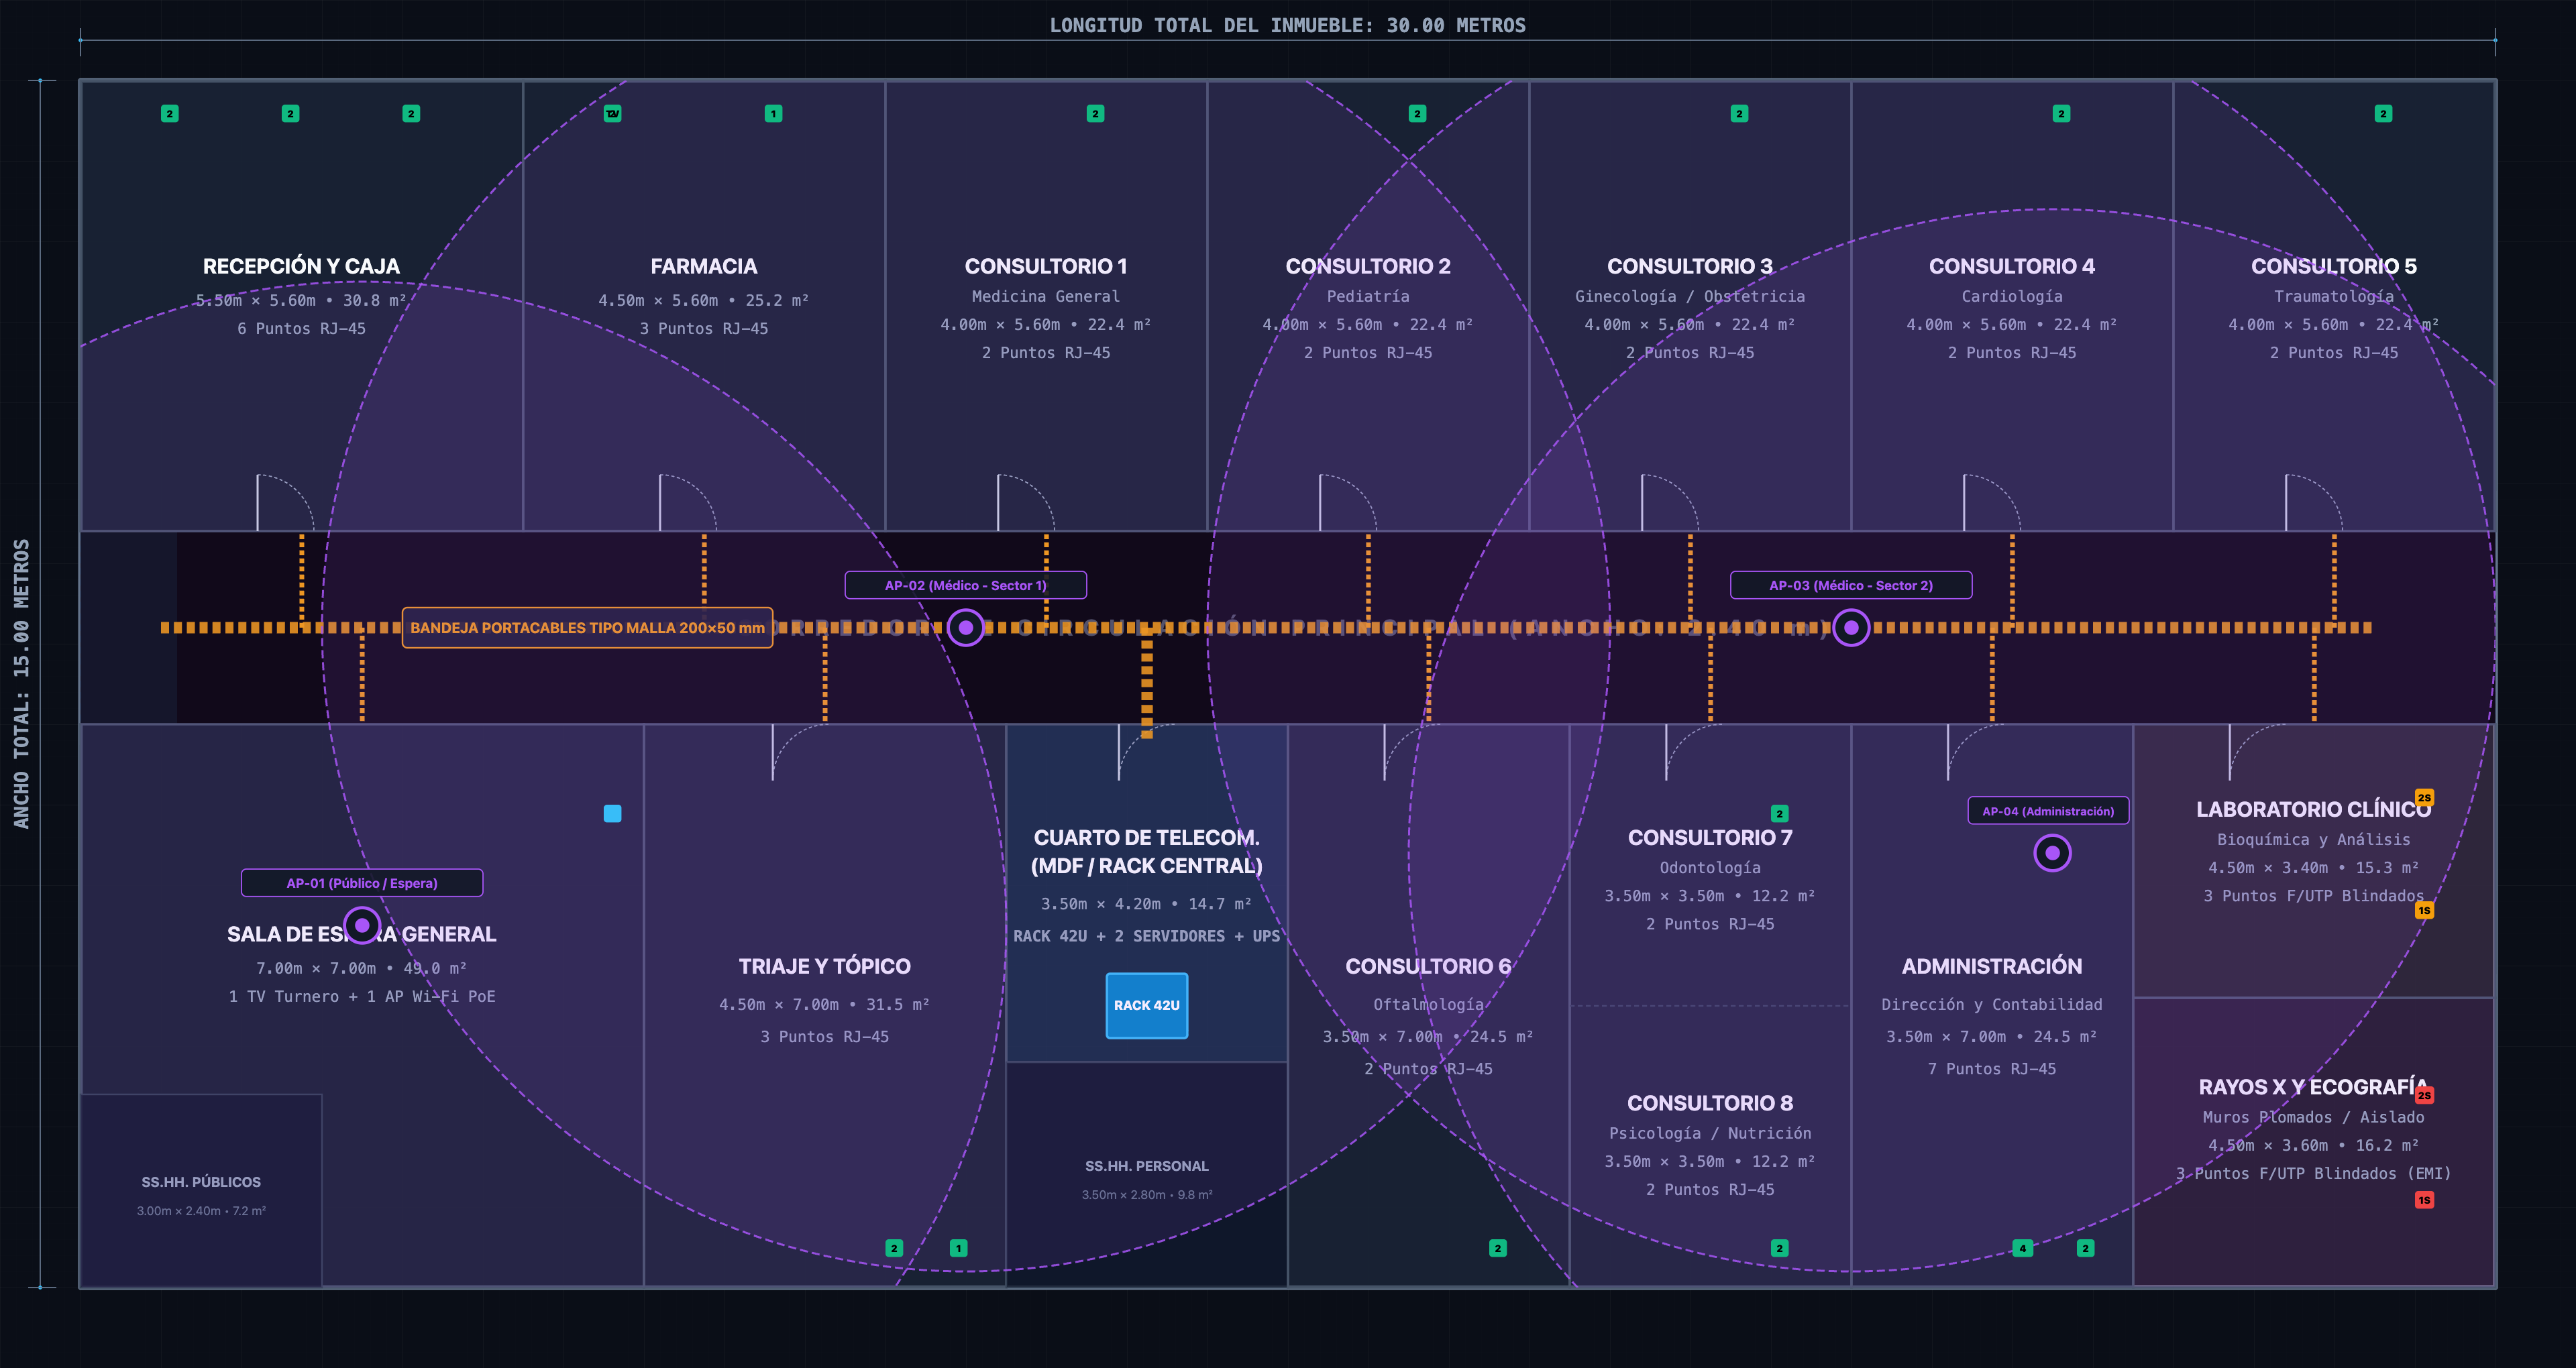
\includegraphics[width=\textwidth]{plano.png}
\caption{Plano arquitectónico civil y distribución espacial de ambientes del Policlínico (Escala 1:100)}
\label{fig:plano-civil}
\end{figure}

\begin{figure}[H]
\centering
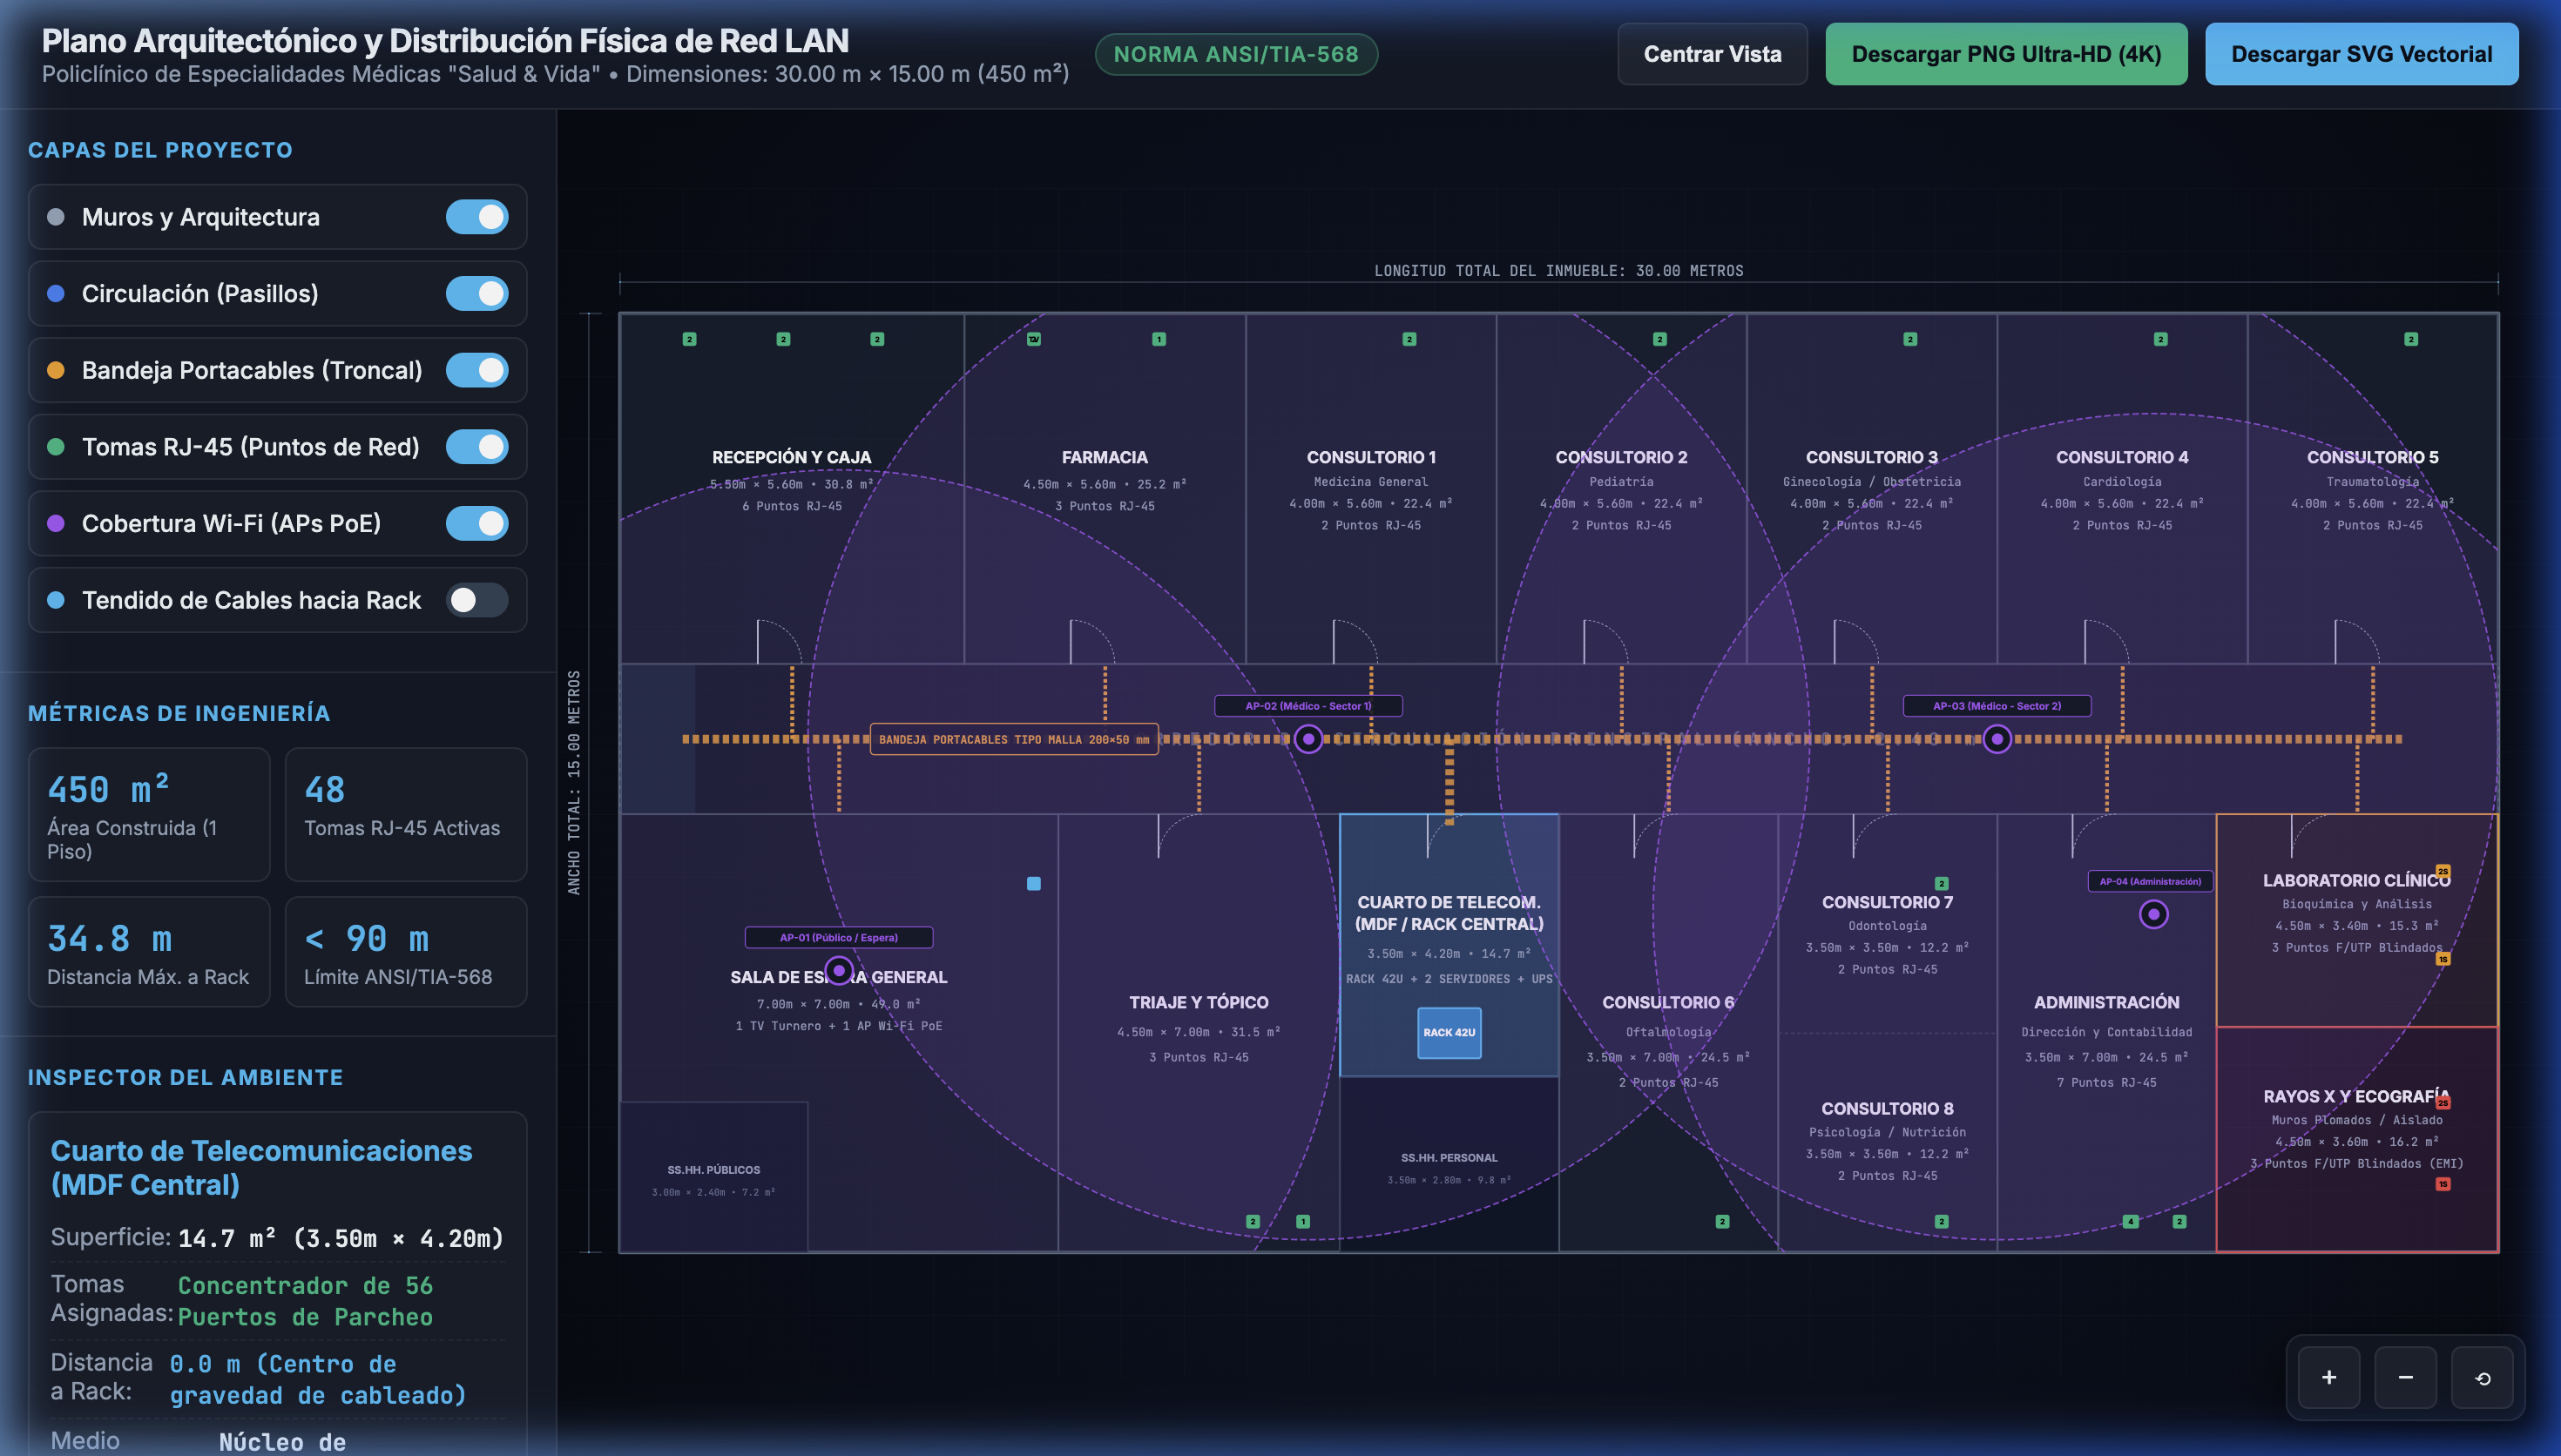
\includegraphics[width=\textwidth]{plano_red_preview.png}
\caption{Plano integral de ingeniería de red LAN: cableado estructurado, canalizaciones y celdas Wi-Fi~6}
\label{fig:plano-red-completo}
\end{figure}

\section{Simbología Normalizada ANSI/TIA-606-B}

\begin{table}[H]
\centering
\caption{Simbología técnica normalizada para planos de red}
\begin{tabularx}{\textwidth}{@{}cclX@{}}
\toprule
\textbf{Símbolo} & \textbf{Código TIA} & \textbf{Componente} & \textbf{Ubicación y Altura} \\
\midrule
$[\bullet\ \bullet]$ & TO-UTP-2  & Toma doble RJ-45 Cat~6 UTP      & Pared a +0.40~m s.n.p.t. / +1.10~m en mesadas \\
$[\blacksquare\ \blacksquare]$  & TO-FTP-2  & Toma doble RJ-45 Cat~6A F/UTP   & Pared a +1.10~m en Lab. y Rayos~X, con tierra \\
$((\text{AP}))$      & WLAN-AP   & Access Point Wi-Fi~6 PoE+       & Anclado en cielo raso a +2.60~m \\
$[\text{TV}]$        & TO-IPTV   & Toma RJ-45 para Smart TV Turnos & Mural a +1.80~m en Sala de Espera \\
$[\text{Rack 42U}]$  & MDF-R1    & Gabinete Rack 42U principal     & Centro geográfico, fijado en losa de concreto \\
$\equiv$             & PATH-BM   & Bandeja malla 200$\times$50~mm  & Suspendida en falso techo a +2.75~m (pasillo) \\
$-\,-\,-$            & PATH-CP   & Canaleta PVC 2 vías 40$\times$25~mm & Adosada a muros a +0.40~m s.n.p.t. \\
\bottomrule
\end{tabularx}
\label{tab:simbologia}
\end{table}

\section{Matriz de Coordenadas y Distancias por Ambiente}

\begin{table}[H]
\centering
\caption{Distancias de enlace permanente por ambiente respecto al MDF}
\small
\begin{tabularx}{\textwidth}{@{} c X c c c c @{}}
\toprule
\textbf{N°} & \textbf{Ambiente} & \textbf{Dim. (m)} & \textbf{Tomas} & \textbf{Dist. Horiz.} & \textbf{Enl. Perm.} \\
\midrule
01 & Recepción / Admisión / Caja        & 5.5$\times$5.6 & 6 UTP   & 13.50~m & 17.70~m \\
02 & Sala de Espera General             & 7.0$\times$7.0 & 2 UTP   & 10.00~m & 14.20~m \\
03 & Triaje y Tópico                    & 4.5$\times$7.0 & 3 UTP   &  6.50~m & 10.70~m \\
04 & Consultorio 01 (Medicina General)  & 4.0$\times$5.6 & 2 UTP   &  4.80~m &  9.00~m \\
05 & Consultorio 02 (Pediatría)         & 4.0$\times$5.6 & 2 UTP   &  6.30~m & 10.50~m \\
06 & Consultorio 03 (Ginecología)       & 4.0$\times$5.6 & 2 UTP   & 10.30~m & 14.50~m \\
07 & Consultorio 04 (Cardiología)       & 4.0$\times$5.6 & 2 UTP   & 14.30~m & 18.50~m \\
08 & Consultorio 05 (Traumatología - Extremo Este) & 4.0$\times$5.6 & 2 UTP & 18.30~m & 22.50~m \\
09 & Consultorio 06 (Oftalmología)      & 3.5$\times$7.0 & 2 UTP   &  6.50~m & 10.70~m \\
10 & Consultorio 07 (Odontología)       & 3.5$\times$3.5 & 2 UTP   &  9.00~m & 13.20~m \\
11 & Consultorio 08 (Psicología)        & 3.5$\times$3.5 & 2 UTP   & 12.00~m & 16.20~m \\
12 & Rayos~X y Ecografía (Zona Crítica) & 4.5$\times$3.6 & 3 F/UTP & 21.00~m & 25.20~m \\
13 & Lab. Clínico (Zona Crítica)        & 4.5$\times$3.4 & 3 F/UTP & 22.00~m & \textbf{34.80~m}$^*$ \\
14 & Farmacia Asistencial               & 4.5$\times$5.6 & 3 UTP   &  9.00~m & 13.20~m \\
15 & Administración / Jefatura          & 3.5$\times$7.0 & 7 UTP   & 15.00~m & 19.20~m \\
16 & Pasillo Central (AP-02 y AP-03)    & 30.0$\times$2.4& 2 PoE   &  7.00~m &  8.50~m \\
17 & Rack MDF (Servidores directos)     & 3.5$\times$4.2 & 3 F/UTP &  1.50~m &  2.50~m \\
18 & Reservas técnicas (distribuidas)   & ---            & 8 UTP   & 18.00~m & 22.20~m \\
\midrule
\multicolumn{3}{l}{\textbf{Total}} & \textbf{56 Tomas} & --- & \textbf{Prom.: 16.5~m} \\
\bottomrule
\multicolumn{6}{@{}p{\textwidth}@{}}{\footnotesize $^*$Toma más lejana (extremo este con retorno ordenado por bandeja). Límite normativo ANSI/TIA-568: $\leq 90.0$~m. Margen de seguridad: +55.2~m (61.3\%).} \\
\end{tabularx}
\label{tab:distancias}
\end{table}

\begin{figure}[H]
\centering
\begin{tikzpicture}[scale=0.45, every node/.style={transform shape}]
    % Perímetro exterior del edificio (30.0m x 15.0m a escala real)
    \draw[line width=1.8pt, fill=gray!3] (0,0) rectangle (30, 15);
    
    % Pasillo central de circulación (X: 0 a 30m, Y: 7.0 a 9.4m -> Ancho 2.4m)
    \draw[fill=yellow!10, draw=gray!40] (0, 7.0) rectangle (30, 9.4);
    \node[font=\bfseries\tiny, text=gray!60] at (15, 8.9) {PASILLO CENTRAL DE CIRCULACIÓN (30.0~m $\times$ 2.4~m)};

    % ========================================================
    % ALA NORTE (Y: 9.4m a 15.0m, Fondo 5.6m) - De Oeste a Este
    % ========================================================
    % 1. Recepción y Caja (0 a 5.5m)
    \draw[line width=1pt, fill=blue!10] (0, 9.4) rectangle (5.5, 15.0);
    \node[align=center, font=\scriptsize\bfseries] at (2.75, 12.2) {RECEPCIÓN\\Y CAJA\\{\tiny 5.5$\times$5.6m}\\{\tiny\color{blue!80!black} 6 Tomas UTP}};

    % 2. Farmacia Asistencial (5.5 a 10.0m)
    \draw[line width=1pt, fill=blue!5] (5.5, 9.4) rectangle (10.0, 15.0);
    \node[align=center, font=\scriptsize] at (7.75, 12.2) {\textbf{FARMACIA}\\{\tiny 4.5$\times$5.6m}\\{\tiny 3 Tomas UTP}};

    % 3. Consultorio 01 - Medicina General (10.0 a 14.0m)
    \draw[line width=1pt] (10.0, 9.4) rectangle (14.0, 15.0);
    \node[align=center, font=\scriptsize] at (12.0, 12.2) {\textbf{C-01}\\{\tiny Med. General}\\{\tiny 4.0$\times$5.6m}\\{\tiny 2 UTP}};

    % 4. Consultorio 02 - Pediatría (14.0 a 18.0m)
    \draw[line width=1pt] (14.0, 9.4) rectangle (18.0, 15.0);
    \node[align=center, font=\scriptsize] at (16.0, 12.2) {\textbf{C-02}\\{\tiny Pediatría}\\{\tiny 4.0$\times$5.6m}\\{\tiny 2 UTP}};

    % 5. Consultorio 03 - Ginecología / Obstetricia (18.0 a 22.0m)
    \draw[line width=1pt] (18.0, 9.4) rectangle (22.0, 15.0);
    \node[align=center, font=\scriptsize] at (20.0, 12.2) {\textbf{C-03}\\{\tiny Ginecología}\\{\tiny 4.0$\times$5.6m}\\{\tiny 2 UTP}};

    % 6. Consultorio 04 - Cardiología (22.0 a 26.0m)
    \draw[line width=1pt] (22.0, 9.4) rectangle (26.0, 15.0);
    \node[align=center, font=\scriptsize] at (24.0, 12.2) {\textbf{C-04}\\{\tiny Cardiología}\\{\tiny 4.0$\times$5.6m}\\{\tiny 2 UTP}};

    % 7. Consultorio 05 - Traumatología (Extremo Este) (26.0 a 30.0m)
    \draw[line width=1pt] (26.0, 9.4) rectangle (30.0, 15.0);
    \node[align=center, font=\scriptsize] at (28.0, 12.2) {\textbf{C-05}\\{\tiny Traumatología}\\{\tiny 4.0$\times$5.6m}\\{\tiny 2 UTP}};

    % ========================================================
    % ALA SUR (Y: 0.0m a 7.0m, Fondo 7.0m) - De Oeste a Este
    % ========================================================
    % 8. Sala de Espera General (0 a 7.0m, Y: 0 a 7.0m)
    \draw[line width=1pt, fill=purple!5] (0, 0) rectangle (7.0, 7.0);
    \draw[fill=gray!25, draw=gray!60] (0, 0) rectangle (3.0, 2.4);
    \node[font=\tiny\bfseries, text=gray!70] at (1.5, 1.2) {SS.HH. PÚBL.};
    \node[align=center, font=\scriptsize\bfseries] at (4.8, 5.5) {SALA DE ESPERA\\GENERAL\\{\tiny 7.0$\times$7.0m (49~m$^2$)}\\{\tiny 2 UTP + Smart TV}};
    % AP-01 UBICADO EXACTAMENTE EN SALA DE ESPERA GENERAL
    \node[circle, fill=purple, text=white, inner sep=2.2pt, font=\bfseries\tiny] (ap1) at (4.0, 3.6) {AP1};
    \draw[purple, dashed, line width=0.9pt] (4.0, 3.6) circle (3.2cm);
    \node[font=\tiny\bfseries, text=purple!90!black, fill=white, inner sep=1pt] at (4.0, 2.9) {AP-01 (Público/Espera)};

    % 9. Triaje y Tópico de Urgencias (7.0 a 11.5m)
    \draw[line width=1pt] (7.0, 0) rectangle (11.5, 7.0);
    \node[align=center, font=\scriptsize] at (9.25, 3.5) {\textbf{TRIAJE Y}\\\textbf{TÓPICO}\\{\tiny 4.5$\times$7.0m}\\{\tiny 3 Tomas UTP}};

    % 10. Cuarto de Comunicaciones (MDF) (11.5 a 15.0m, Y: 2.8 a 7.0m)
    \draw[line width=1.6pt, fill=teal!20, draw=teal!80!black] (11.5, 2.8) rectangle (15.0, 7.0);
    \node[align=center, font=\scriptsize\bfseries, text=teal!90!black, fill=teal!20, inner sep=1pt] at (13.25, 5.8) {CUARTO MDF\\{\tiny 3.5$\times$4.2m}\\{\tiny 3 Servidores}};
    \draw[fill=black] (12.4, 3.4) rectangle (14.1, 4.6);
    \node[text=white, font=\tiny\bfseries] at (13.25, 4.0) {RACK 42U};
    \draw[fill=gray!25, draw=gray!60] (11.5, 0) rectangle (15.0, 2.8);
    \node[font=\tiny\bfseries, text=gray!70] at (13.25, 1.4) {SS.HH. PERSONAL};

    % 11. Consultorio 06 - Oftalmología (15.0 a 18.5m)
    \draw[line width=1pt] (15.0, 0) rectangle (18.5, 7.0);
    \node[align=center, font=\scriptsize] at (16.75, 3.5) {\textbf{C-06}\\{\tiny Oftalmología}\\{\tiny 3.5$\times$7.0m}\\{\tiny 2 UTP}};

    % 12. Consultorios 07 y 08 (18.5 a 22.0m)
    \draw[line width=1pt] (18.5, 3.5) rectangle (22.0, 7.0);
    \node[align=center, font=\scriptsize, fill=white, inner sep=0.8pt] at (20.25, 5.25) {\textbf{C-07}\\{\tiny Odontol.}\\{\tiny 3.5$\times$3.5m}\\{\tiny 2 UTP}};
    \draw[line width=1pt] (18.5, 0) rectangle (22.0, 3.5);
    \node[align=center, font=\scriptsize, fill=white, inner sep=0.8pt] at (20.25, 1.75) {\textbf{C-08}\\{\tiny Psicología}\\{\tiny 3.5$\times$3.5m}\\{\tiny 2 UTP}};

    % 13. Administración y Jefatura Médica (22.0 a 25.5m)
    \draw[line width=1pt, fill=green!8] (22.0, 0) rectangle (25.5, 7.0);
    \node[align=center, font=\scriptsize, fill=green!8, inner sep=0.8pt] at (23.75, 2.2) {\textbf{ADMINISTRACIÓN}\\{\tiny Dirección / Contab.}\\{\tiny 3.5$\times$7.0m}\\{\tiny 7 Tomas UTP}};
    % AP-04 UBICADO EN ADMINISTRACIÓN
    \node[circle, fill=purple, text=white, inner sep=2.2pt, font=\bfseries\tiny] (ap4) at (23.75, 5.4) {AP4};
    \draw[purple, dashed, line width=0.9pt] (23.75, 5.4) circle (3.2cm);
    \node[font=\tiny\bfseries, text=purple!90!black, fill=white, inner sep=1pt] at (23.75, 4.6) {AP-04 (Admin)};

    % 14. Zona Crítica EMI (25.5 a 30.0m)
    % Laboratorio Clínico (Arriba)
    \draw[line width=1.2pt, fill=orange!15, draw=orange!80!black] (25.5, 3.6) rectangle (30.0, 7.0);
    \node[align=center, font=\scriptsize\bfseries, text=orange!90!black] at (27.75, 5.3) {LABORATORIO\\CLÍNICO\\{\tiny 4.5$\times$3.4m}\\{\tiny 3 F/UTP Blindados}\\\textbf{\tiny Enlace: 34.8~m max}};
    % Rayos X y Ecografía (Abajo)
    \draw[line width=1.2pt, fill=red!15, draw=red!80!black] (25.5, 0) rectangle (30.0, 3.6);
    \node[align=center, font=\scriptsize\bfseries, text=red!90!black] at (27.75, 1.8) {RAYOS X Y\\ECOGRAFÍA\\{\tiny Sala Plomada (EMI)}\\{\tiny 4.5$\times$3.6m}\\{\tiny 3 F/UTP Blindados}};

    % ========================================================
    % BANDEJA TIPO MALLA PORTACABLES Y ACCES POINT EN PASILLO
    % ========================================================
    \draw[line width=2.4pt, color=orange!85!black, dashed] (1.0, 8.2) -- (29.0, 8.2);
    \draw[line width=2.4pt, color=orange!85!black, dashed] (13.25, 8.2) -- (13.25, 4.6);
    \node[font=\bfseries\tiny, text=orange!90!black, fill=white, inner sep=1.2pt, rounded corners=1pt] at (6.0, 8.2) {Bandeja Malla 200$\times$50~mm (Cielo Raso)};

    % AP-02 (Pasillo Central Oeste - Sector Médico 1)
    \node[circle, fill=purple, text=white, inner sep=2.2pt, font=\bfseries\tiny] (ap2) at (11.0, 7.8) {AP2};
    \draw[purple, dashed, line width=0.9pt] (11.0, 7.8) circle (3.2cm);
    \node[font=\tiny\bfseries, text=purple!90!black, fill=white, inner sep=1pt] at (11.0, 8.6) {AP-02 (Médico Oeste)};

    % AP-03 (Pasillo Central Este - Sector Médico 2)
    \node[circle, fill=purple, text=white, inner sep=2.2pt, font=\bfseries\tiny] (ap3) at (22.5, 7.8) {AP3};
    \draw[purple, dashed, line width=0.9pt] (22.5, 7.8) circle (3.2cm);
    \node[font=\tiny\bfseries, text=purple!90!black, fill=white, inner sep=1pt] at (22.5, 8.6) {AP-03 (Médico Este)};

    % Cotas perimetrales
    \draw[{Latex[length=2mm]}-{Latex[length=2mm]}, line width=0.8pt] (0, 15.5) -- (30, 15.5);
    \node[font=\tiny\bfseries] at (15, 15.9) {LONGITUD TOTAL DEL INMUEBLE: 30.00 METROS};

    \draw[{Latex[length=2mm]}-{Latex[length=2mm]}, line width=0.8pt] (-0.6, 0) -- (-0.6, 15);
    \node[font=\tiny\bfseries, rotate=90] at (-1.0, 7.5) {ANCHO TOTAL: 15.00 METROS};

    % Leyenda técnica inferior
    \node[draw, fill=white, rounded corners=2pt, font=\scriptsize, align=left] at (15, -1.8) {
        \textbf{Leyenda de Infraestructura:} \quad
        {\color{orange!85!black}\textbf{-- --}} Bandeja portacables tipo malla 200$\times$50~mm \quad
        \textbf{[$\bullet$]} Jacks UTP Cat~6 \quad
        {\color{red!70}\textbf{[$\blacksquare$]}} Puntos F/UTP Cat~6A blindados \quad
        {\color{purple}\textbf{((AP))}} AP Wi-Fi~6 PoE+
    };
\end{tikzpicture}
\caption{Plano esquemático arquitectónico y distribución física de ambientes, canalizaciones y Access Points Wi-Fi~6}
\label{fig:planoesquematico}
\end{figure}

\section{Diseño de Cobertura Inalámbrica Wi-Fi 6}

\subsection{Criterios de Propagación en Banda de 5 GHz}

\begin{itemize}[leftmargin=*]
    \item \textbf{Radio de célula efectivo:} 8.0~m en espacio semiabierto hospitalario.
    \item \textbf{RSSI en borde de célula:} $\geq -65~\text{dBm}$, garantizando modulaciones MCS altas y tasas reales superiores a 150~Mbps por usuario.
    \item \textbf{Solapamiento entre APs adyacentes:} 15\%, garantizando \textit{Fast Roaming} (802.11r/k/v) sin corte de sesión.
    \item \textbf{Separación de redes (SSID):}
    \begin{itemize}
        \item \textit{SSID Médico (``Salud\_Clinica''):} WPA3-Enterprise, prioridad QoS-WMM para VoIP y EMR.
        \item \textit{SSID Público (``Salud\_Pacientes''):} Aislado de la red interna, ancho de banda limitado por usuario.
    \end{itemize}
\end{itemize}

\subsection{Ubicación y Cobertura de los Cuatro APs}

\begin{table}[H]
\centering
\caption{Distribución y cobertura de los Access Points Wi-Fi~6}
\small
\begin{tabularx}{\textwidth}{@{}clXl@{}}
\toprule
\textbf{AP} & \textbf{Ubicación Física} & \textbf{Cobertura Funcional} & \textbf{Código PP} \\
\midrule
AP-01 & Sala de Espera General     & Red pública de pacientes y pantalla de turnos & PP01-08 \\
AP-02 & Pasillo Central Oeste      & Médica: Consultorios 1--4 y Triaje (Roaming) & PP02-14 \\
AP-03 & Pasillo Central Este       & Médica: Consultorios 5--8 y Laboratorio       & PP02-15 \\
AP-04 & Administración (Sector E)  & Corporativa: Jefatura, Contabilidad, Estar Médico & PP02-13 \\
\bottomrule
\end{tabularx}
\label{tab:aps}
\end{table}

\section{BOM Valorizado y Presupuesto Referencial}

Los precios corresponden a mercado institucional en Perú (distribuidores Panduit, Siemon, Cisco, APC) a tipo de cambio referencial de \textbf{S/.~3.75 por USD}.

\subsection{Partida 01: Infraestructura Pasiva de Cableado}

\begin{table}[H]
\centering
\caption{Partida 01 --- Infraestructura pasiva y conectividad}
\small
\begin{tabularx}{\textwidth}{@{} c X c c r r @{}}
\toprule
\textbf{Ítem} & \textbf{Descripción} & \textbf{Cant.} & \textbf{Ud.} & \textbf{P.Unit. (USD)} & \textbf{Subtotal (USD)} \\
\midrule
1.1  & Cable UTP Cat~6 LSZH (305~m)            & 4  & Rollo & \$195.00 & \$780.00 \\
1.2  & Cable F/UTP Cat~6A Blindado (305~m)     & 1  & Rollo & \$340.00 & \$340.00 \\
1.3  & Jack Keystone Cat~6 UTP                 & 50 & Pza   & \$3.80   & \$190.00 \\
1.4  & Jack Keystone Cat~6A Blindado           & 6  & Pza   & \$8.50   & \$51.00  \\
1.5  & Faceplate 2 ventanas                    & 23 & Pza   & \$2.20   & \$50.60  \\
1.6  & Faceplate 4 ventanas                    & 2  & Pza   & \$3.50   & \$7.00   \\
1.7  & Patch Cord UTP Cat~6 2.0~m              & 46 & Pza   & \$4.20   & \$193.20 \\
1.8  & Patch Cord UTP Cat~6 1.0~m (rack)       & 50 & Pza   & \$3.10   & \$155.00 \\
1.9  & Patch Cord F/UTP Cat~6A 2.0~m           & 6  & Pza   & \$7.80   & \$46.80  \\
1.10 & Patch Cord F/UTP Cat~6A 1.0~m (rack)    & 6  & Pza   & \$5.90   & \$35.40  \\
1.11 & Patch Panel 24p Cat~6 UTP 19''          & 2  & Pza   & \$85.00  & \$170.00 \\
1.12 & Patch Panel 24p Cat~6A Blindado         & 1  & Pza   & \$135.00 & \$135.00 \\
1.13 & Organizador horizontal 1U 19''          & 3  & Pza   & \$18.00  & \$54.00  \\
\midrule
\multicolumn{5}{r}{\textbf{SUBTOTAL Partida 01}} & \textbf{\$2,208.00} \\
\bottomrule
\end{tabularx}
\label{tab:partida01}
\end{table}

\subsection{Partida 02: Canalizaciones y Puesta a Tierra}

\begin{table}[H]
\centering
\caption{Partida 02 --- Canalizaciones y sistema de tierra}
\small
\begin{tabularx}{\textwidth}{@{} c X c c r r @{}}
\toprule
\textbf{Ítem} & \textbf{Descripción} & \textbf{Cant.} & \textbf{Ud.} & \textbf{P.Unit. (USD)} & \textbf{Subtotal (USD)} \\
\midrule
2.1 & Bandeja malla cincada 200$\times$50~mm (tramos 3~m) & 10 & Tramo & \$32.00  & \$320.00 \\
2.2 & Kit accesorios para bandeja (uniones, grapas)        & 1  & Glb   & \$85.00  & \$85.00  \\
2.3 & Varilla roscada 3/8'' + tacos + tuercas              & 12 & Juego & \$6.50   & \$78.00  \\
2.4 & Canaleta PVC 2 vías 40$\times$25~mm (tramos 2~m)    & 45 & Tramo & \$8.40   & \$378.00 \\
2.5 & Accesorios canaleta (esquineros, tes, uniones)       & 1  & Glb   & \$65.00  & \$65.00  \\
2.6 & Barra TMGB de cobre 10$\times$50$\times$300~mm      & 1  & Pza   & \$110.00 & \$110.00 \\
2.7 & Cable de tierra cobre AWG~6 (15~m)                   & 1  & Rollo & \$48.00  & \$48.00  \\
\midrule
\multicolumn{5}{r}{\textbf{SUBTOTAL Partida 02}} & \textbf{\$1,084.00} \\
\bottomrule
\end{tabularx}
\label{tab:partida02}
\end{table}

\subsection{Partida 03: Gabinete Rack, Respaldo Eléctrico y Climatización}

\begin{table}[H]
\centering
\caption{Partida 03 --- Rack, UPS y climatización}
\small
\begin{tabularx}{\textwidth}{@{} c X c c r r @{}}
\toprule
\textbf{Ítem} & \textbf{Descripción} & \textbf{Cant.} & \textbf{Ud.} & \textbf{P.Unit. (USD)} & \textbf{Subtotal (USD)} \\
\midrule
3.1 & Gabinete Rack 42U 19'', profundidad 800~mm            & 1 & Pza & \$750.00  & \$750.00  \\
3.2 & PDU horizontal 1U, 8 tomas C13 con switch térmico     & 1 & Pza & \$75.00   & \$75.00   \\
3.3 & UPS Online Doble Conversión 3000~VA / 2700~W (3U)     & 1 & Pza & \$1,150.00 & \$1,150.00 \\
3.4 & Banco baterías extendido para UPS (3U, 45~min)        & 1 & Pza & \$580.00  & \$580.00  \\
3.5 & Bandeja 4 extractores de aire 220~VAC con termostato  & 1 & Pza & \$95.00   & \$95.00   \\
\midrule
\multicolumn{5}{r}{\textbf{SUBTOTAL Partida 03}} & \textbf{\$2,650.00} \\
\bottomrule
\end{tabularx}
\label{tab:partida03}
\end{table}

\subsection{Partida 04: Equipamiento Activo de Red y WLAN}

\begin{table}[H]
\centering
\caption{Partida 04 --- Equipamiento activo y conectividad inalámbrica}
\small
\begin{tabularx}{\textwidth}{@{} c X c c r r @{}}
\toprule
\textbf{Ítem} & \textbf{Descripción} & \textbf{Cant.} & \textbf{Ud.} & \textbf{P.Unit. (USD)} & \textbf{Subtotal (USD)} \\
\midrule
4.1 & Switch L2 Adm. 24p GbE PoE+ (370W) + 4 SFP+~10G  & 2 & Pza & \$820.00 & \$1,640.00 \\
4.2 & Switch Core/Distribución 24p GbE + 4 SFP+~10G     & 1 & Pza & \$950.00 & \$950.00   \\
4.3 & Cable DAC pasivo SFP+~10G de 1.0~m (uplinks)      & 4 & Pza & \$35.00  & \$140.00   \\
4.4 & Access Point Wi-Fi~6 (802.11ax) Dual Band PoE+    & 4 & Pza & \$240.00 & \$960.00   \\
\midrule
\multicolumn{5}{r}{\textbf{SUBTOTAL Partida 04}} & \textbf{\$3,690.00} \\
\bottomrule
\end{tabularx}
\label{tab:partida04}
\end{table}

\subsection{Resumen General del Presupuesto}

\begin{table}[H]
\centering
\caption{Resumen consolidado del presupuesto de infraestructura}
\small
\begin{tabularx}{\textwidth}{@{} c X r r r @{}}
\toprule
\textbf{Partida} & \textbf{Descripción del Rubro} & \textbf{Subtotal (USD)} & \textbf{Subtotal (PEN)} & \textbf{Incidencia} \\
\midrule
01 & Infraestructura Pasiva de Cableado   & \$2,208.00 & S/.~8,280.00  & 22.92\% \\
02 & Canalizaciones y Puesta a Tierra     & \$1,084.00 & S/.~4,065.00  & 11.25\% \\
03 & Gabinete, UPS y Climatización        & \$2,650.00 & S/.~9,937.50  & 27.52\% \\
04 & Equipamiento Activo y WLAN           & \$3,690.00 & S/.~13,837.50 & 38.31\% \\
\midrule
\textbf{TOTAL} & \textbf{Costo Total Directo de Suministros} & \textbf{\$9,632.00} & \textbf{S/.~36,120.00} & \textbf{100.00\%} \\
\bottomrule
\end{tabularx}
\label{tab:presupuesto-total}
\end{table}

\section{Plan de Mantenimiento Preventivo Físico}

\begin{table}[H]
\centering
\caption{Calendario de mantenimiento preventivo de la infraestructura}
\small
\begin{tabularx}{\textwidth}{@{}clX@{}}
\toprule
\textbf{Frecuencia} & \textbf{Actividad} & \textbf{Descripción} \\
\midrule
Trimestral  & Limpieza de rack          & Filtros y ventiladores del techo del rack 42U; monitoreo térmico (18--24°C). \\
Semestral   & Inspección de bandeja     & Verificación visual en cielo raso; control de peinado de patch cords en 1U. \\
Anual       & Tierra de telecomunicaciones & Medición con telurómetro: resistencia $\leq 5~\Omega$ (TIA-607-C); reapriete de cables de drenaje. \\
Bianual     & Re-certificación aleatoria & 10\% de enlaces permanentes con Fluke DSX-5000/8000 CableAnalyzer. \\
\bottomrule
\end{tabularx}
\label{tab:mantenimiento}
\end{table}

\chapter{Construcción de Cable UTP y Plan de Pruebas de Certificación}

\section{Introducción y Objetivos}

La presente etapa constituye el componente de validación empírica y aseguramiento normativo del proyecto. Define:

\begin{enumerate}[leftmargin=*, label=\arabic*.]
    \item El protocolo metrológico de certificación de los 56 enlaces permanentes bajo la norma \textbf{ANSI/TIA-568-C.2}.
    \item El procedimiento exhaustivo de manufactura artesanal de la muestra física de cable UTP Cat~6 bajo la norma \textbf{T568B}.
    \item La taxonomía de fallas de cableado y el análisis del par dividido (\textit{Split Pair}).
    \item La guía de preparación para la evaluación individual aleatoria ante el docente.
    \item El formato formal de Hoja de Reporte de Certificación (\textit{Test Report Sheet}).
\end{enumerate}

\section{Plan de Pruebas y Certificación de Enlace Permanente}

\subsection{Enlace Permanente vs. Canal Completo}

La norma \textbf{ANSI/TIA-568.0-D} define dos configuraciones de medición con tolerancias distintas:

\begin{table}[H]
\caption{Diferenciación entre Enlace Permanente y Canal Completo}
\begin{tabularx}{\textwidth}{@{}lXX@{}}
\toprule
\textbf{Criterio} & \textbf{Enlace Permanente (\textit{Permanent Link})} & \textbf{Canal Completo (\textit{Channel})} \\
\midrule
Definición        & Infraestructura fija desde el terminal IDC del Patch Panel hasta el jack Keystone de pared & Enlace permanente más los dos latiguillos de ambos extremos \\
Longitud Máxima   & \textbf{90.0~m estrictos} & \textbf{100.0~m totales} ($90 + 10$~m de patch cords) \\
Exclusión         & El instrumento descuenta automáticamente sus adaptadores & Evalúa toda la ruta incluyendo conectores terminales \\
Uso en el Proyecto & \textbf{Modelo obligatorio para certificación y entrega de obra} (garantía 20 años) & Usado durante mantenimiento operativo \\
\bottomrule
\end{tabularx}
\label{tab:permanentlink}
\end{table}

\subsection{Parámetros Eléctricos y de RF Certificados (TIA-568-C.2)}

Cada uno de los 56 enlaces (50 UTP Cat~6 + 6 F/UTP Cat~6A) es sometido al barrido del certificador de campo Nivel~IIIe (\textit{Fluke DSX-5000 / DSX-8000}):

\begin{table}[H]
\caption{Parámetros de certificación y valores límite --- Cat~6 a 250~MHz}
\begin{tabularx}{\textwidth}{@{}lXcc@{}}
\toprule
\textbf{Parámetro} & \textbf{Descripción} & \textbf{Límite TIA Cat~6} & \textbf{Causa Típica de Falla} \\
\midrule
\textit{Wire Map}       & Continuidad pin a pin + pantalla (Cat~6A)              & 1:1 Continuo  & Error de pinout, corte al desforrar \\
\textit{Length (TDR)}   & Longitud medida por reflectometría (NVP $\approx 0.69c$)& $\leq 90.0$~m & Tirada excesiva de cable \\
\textit{IL} (Atenuación)& Pérdida de potencia de señal a 250~MHz                  & $\leq 31.1$~dB & Cable CCA o longitud excesiva \\
\textit{NEXT}           & Paradiafonía: inducción entre pares en extremo cercano  & $\geq 35.3$~dB & Destrenzado $>$ 13~mm al terminar \\
\textit{PS-NEXT}        & Suma de potencia de diafonía de 3 pares sobre el 4°     & $\geq 32.7$~dB & Precintos demasiado ajustados \\
\textit{Return Loss}    & Energía reflejada por variaciones de impedancia (100~$\Omega$) & $\geq 10.0$~dB & Quiebre por debajo del radio mínimo ($4\times$OD) \\
\textit{Delay / Skew}   & Tiempo de arribo y diferencia entre par más rápido/lento & Skew $\leq 45$~ns & Torsión despareja de fábrica \\
\bottomrule
\end{tabularx}
\label{tab:certificacion}
\end{table}

\subsubsection{Cálculo de Atenuación en el Enlace Más Lejano}

Para el enlace del Laboratorio Clínico (34.80~m), la atenuación estimada por la fórmula de la norma TIA es:

\begin{equation}
IL(250~\text{MHz}) \approx 32~\frac{\text{dB}}{100~\text{m}} \times \frac{34.80~\text{m}}{100~\text{m}} \approx 11.14~\text{dB}
\end{equation}

Esto genera un \textbf{margen favorable (\textit{headroom})} de casi 20~dB sobre el límite máximo de 31.1~dB.

\subsection{Diagnóstico de Fallas y el Par Dividido (\textit{Split Pair})}

\begin{table}[H]
\caption{Tipología de fallas en ensayos de cableado de par trenzado}
\begin{tabularx}{\textwidth}{@{}lXl@{}}
\toprule
\textbf{Tipo de Falla} & \textbf{Descripción} & \textbf{Detección} \\
\midrule
Circuito Abierto (\textit{Open})    & Conductor cortado o sin contacto en la cuchilla IDC            & Tester LED / Certificador \\
Cortocircuito (\textit{Short})      & Dos conductores en contacto eléctrico indeseado                & Tester LED / Certificador \\
Par Invertido (\textit{Reversed})   & Pines 1 y 2 intercambiados en un extremo                       & Tester LED / Certificador \\
Par Cruzado (\textit{Crossed})      & Un par entero en posiciones de otro                             & Tester LED / Certificador \\
\textbf{Par Dividido (\textit{Split Pair})} & Hilos de distintos pares mezclados idénticamente en ambos extremos & \textbf{Solo Certificador RF} \\
\bottomrule
\end{tabularx}
\label{tab:fallas}
\end{table}

El \textbf{par dividido} es la falla más peligrosa: un tester básico de LEDs muestra continuidad aparente 1:1 (falso aprobado), pero en la transmisión real la geometría de par trenzado balanceado se rompe, generando un \textbf{NEXT catastrófico de 10 a 15~dB} que impide la negociación Gigabit y provoca hasta el 80\% de pérdida de paquetes.

\begin{figure}[H]
\centering
\begin{tikzpicture}[scale=0.88, every node/.style={transform shape}]
    % Caso A: Cableado Normal (T568B)
    \node[font=\bfseries\small, text=mdpiBlue] at (3.5, 4.3) {A) Cableado Correcto T568B (Pares Balanceados)};
    \draw[fill=gray!10, rounded corners] (-0.3, -0.4) rectangle (7.3, 3.8);

    % Pines Extremo A y Extremo B
    \foreach \i in {1,...,8} {
        \node[circle, fill=black, text=white, inner sep=1.5pt, font=\tiny\bfseries] (A\i) at (0.5, 3.9 - 0.45*\i) {\i};
        \node[circle, fill=black, text=white, inner sep=1.5pt, font=\tiny\bfseries] (B\i) at (6.5, 3.9 - 0.45*\i) {\i};
    }
    % Líneas de pares
    \draw[line width=1.5pt, orange] (A1) -- (B1);
    \draw[line width=1.5pt, orange!70!black] (A2) -- (B2);
    \draw[line width=1.5pt, green!60!black] (A3) -- (B3);
    \draw[line width=1.5pt, blue] (A4) -- (B4);
    \draw[line width=1.5pt, blue!70!black] (A5) -- (B5);
    \draw[line width=1.5pt, green!60!black] (A6) -- (B6);
    \draw[line width=1.5pt, brown] (A7) -- (B7);
    \draw[line width=1.5pt, brown!70!black] (A8) -- (B8);

    \node[right, font=\tiny, text=green!60!black] at (2.2, 0.3) {NEXT $>$ 35~dB: \textbf{APROBADO}};

    % Caso B: Par Dividido (Split Pair)
    \begin{scope}[xshift=8.5cm]
        \node[font=\bfseries\small, text=red!80!black] at (3.5, 4.3) {B) Par Dividido / Split Pair (Falso Aprobado en LED)};
        \draw[fill=red!5, draw=red!40, rounded corners] (-0.3, -0.4) rectangle (7.3, 3.8);

        \foreach \i in {1,...,8} {
            \node[circle, fill=black, text=white, inner sep=1.5pt, font=\tiny\bfseries] (SA\i) at (0.5, 3.9 - 0.45*\i) {\i};
            \node[circle, fill=black, text=white, inner sep=1.5pt, font=\tiny\bfseries] (SB\i) at (6.5, 3.9 - 0.45*\i) {\i};
        }
        % Continuidad DC es 1:1
        \draw[line width=1.5pt, orange] (SA1) -- (SB1);
        \draw[line width=1.5pt, orange!70!black] (SA2) -- (SB2);
        % Error: Hilo de Par 3 mezclado en vaina con hilo de Par 1
        \draw[line width=1.5pt, red, dashed] (SA3) -- (SB3);
        \draw[line width=1.5pt, red, dashed] (SA4) -- (SB4);
        \draw[line width=1.5pt, blue!70!black] (SA5) -- (SB5);
        \draw[line width=1.5pt, green!60!black] (SA6) -- (SB6);
        \draw[line width=1.5pt, brown] (SA7) -- (SB7);
        \draw[line width=1.5pt, brown!70!black] (SA8) -- (SB8);

        \draw[{Latex[length=2mm]}-{Latex[length=2mm]}, red, line width=1pt] (3.5, 2.5) -- (3.5, 2.1);
        \node[font=\tiny\bfseries, text=red] at (3.5, 1.8) {Fuerte acoplamiento RF};
        \node[right, font=\tiny, text=red] at (1.8, 0.3) {NEXT $< 15$~dB: \textbf{FALLA CRÍTICA}};
    \end{scope}
\end{tikzpicture}
\caption{Comparativa entre canal balanceado T568B y defecto electromagnético de Par Dividido (\textit{Split Pair})}
\label{fig:splitpair}
\end{figure}

\begin{figure}[H]
\centering
\begin{tikzpicture}[scale=1.1]
    % Chaqueta exterior LSZH
    \draw[fill=blue!10, draw=blue!70, line width=2pt] (0,0) circle (2.2cm);
    \node[font=\tiny\bfseries, text=blue!80] at (0, 2.45) {Chaqueta exterior LSZH (Ø 6.2 mm)};

    % Cruceta plástica separadora central (Spline)
    \draw[fill=gray!30, draw=gray!70, line width=1pt] (-0.25, -1.8) rectangle (0.25, 1.8);
    \draw[fill=gray!30, draw=gray!70, line width=1pt] (-1.8, -0.25) rectangle (1.8, 0.25);
    \node[font=\tiny\bfseries, text=gray!80] at (0, 0) {Spline PE};

    % Hilo de rasgado (Rip cord)
    \fill[red] (1.3, 1.3) circle (2pt);
    \node[font=\tiny, text=red!80, anchor=west] at (1.4, 1.4) {Rip cord};

    % Par 2 (Naranja) - Superior Izquierda
    \draw[fill=orange!30, draw=orange!90, line width=0.8pt] (-1.0, 1.0) circle (0.42cm);
    \draw[fill=orange!90, draw=orange!90, line width=0.8pt] (-0.8, 0.8) circle (0.22cm);
    \node[font=\tiny\bfseries] at (-1.0, 1.55) {Par 2 (B/N - N)};

    % Par 1 (Azul) - Superior Derecha
    \draw[fill=blue!30, draw=blue!90, line width=0.8pt] (1.0, 0.9) circle (0.42cm);
    \draw[fill=blue!90, draw=blue!90, line width=0.8pt] (0.8, 0.7) circle (0.22cm);
    \node[font=\tiny\bfseries] at (1.0, 1.55) {Par 1 (B/A - A)};

    % Par 3 (Verde) - Inferior Izquierda
    \draw[fill=green!30, draw=green!70!black, line width=0.8pt] (-1.0, -1.0) circle (0.42cm);
    \draw[fill=green!70!black, draw=green!70!black, line width=0.8pt] (-0.8, -0.8) circle (0.22cm);
    \node[font=\tiny\bfseries] at (-1.0, -1.65) {Par 3 (B/V - V)};

    % Par 4 (Marrón) - Inferior Derecha
    \draw[fill=brown!35, draw=brown!80!black, line width=0.8pt] (1.0, -1.0) circle (0.42cm);
    \draw[fill=brown!80!black, draw=brown!90!black, line width=0.8pt] (0.8, -0.8) circle (0.22cm);
    \node[font=\tiny\bfseries] at (1.0, -1.65) {Par 4 (B/M - M)};
\end{tikzpicture}
\caption{Corte transversal y anatomía física del cable UTP Categoría 6 monofilamento 23~AWG}
\label{fig:cablecat6}
\end{figure}

\section{Guía de Fabricación de la Muestra Física UTP (T568B)}

\subsection{Materiales Necesarios}

\begin{itemize}[leftmargin=*]
    \item 2.0~m de cable UTP Cat~6 monofilamento 23~AWG, 100\% cobre, forro LSZH.
    \item 2 conectores machos RJ-45 (8P8C) Cat~6 con contactos dorados de 50~$\mu$in y guía escalonada.
    \item 2 capuchones de goma termoplástica protectores de lengüeta.
    \item Herramienta pelacables rotativa, ponchadora de trinquete y tester de continuidad.
\end{itemize}

\subsection{Procedimiento Paso a Paso}

\begin{enumerate}[leftmargin=*, label=\textbf{Paso \arabic*.}]
    \item \textbf{Capuchones:} Deslizar un capuchón en cada extremo del cable (sentido invertido) \textit{antes} de desforrar.
    
    \item \textbf{Desforrado:} Retirar exactamente \textbf{30~mm} de chaqueta exterior con la herramienta pelacables calibrada, sin mellar el aislamiento interno de los 8 conductores.
    
    \item \textbf{Retiro de elementos pasivos:} Cortar al ras con alicate diagonal el hilo de rasgado (\textit{rip cord}) y el separador cruciforme (\textit{spline}).
    
    \item \textbf{Ordenamiento T568B:} Destrenzar los pares \textbf{no más de 13~mm} desde la chaqueta. Ordenar de izquierda a derecha (pestaña del conector hacia abajo):
    \begin{equation*}
        \underbrace{\text{B/Naranja}}_{\text{Pin 1}} - \underbrace{\text{Naranja}}_{\text{Pin 2}} - \underbrace{\text{B/Verde}}_{\text{Pin 3}} - \underbrace{\text{Azul}}_{\text{Pin 4}} - \underbrace{\text{B/Azul}}_{\text{Pin 5}} - \underbrace{\text{Verde}}_{\text{Pin 6}} - \underbrace{\text{B/Marrón}}_{\text{Pin 7}} - \underbrace{\text{Marrón}}_{\text{Pin 8}}
    \end{equation*}
    
    \item \textbf{Corte a 90°:} Recortar con corte perpendicular dejando \textbf{13 a 14~mm} de conductores expuestos desde la chaqueta.
    
    \item \textbf{Inserción:} Deslizar en el conector RJ-45 hasta que los 8 conductores toquen visualmente el frente transparente. \textbf{Criterio crítico:} la chaqueta debe ingresar al menos \textbf{6~mm} dentro del cuerpo del conector para ser prensada por la cuña de retención mecánica.
    
    \item \textbf{Crimpado:} Colocar en el puerto 8P de la ponchadora de trinquete y presionar hasta liberar el seguro. Las 8 cuchillas doradas perforan el aislamiento por desplazamiento (\textit{IDC}).
    
    \item \textbf{Verificación:} Conectar a tester de continuidad (Master + Remote). Los LEDs del 1 al 8 deben encenderse en \textbf{secuencia sincrónica y verde}, confirmando la ausencia de cortes, pares cruzados o falsos contactos.
\end{enumerate}

\section{Guía para la Evaluación Individual Aleatoria}

\subsection{Preguntas Típicas de Sustentación y Respuestas Esperadas}

\subsubsection{¿Por qué se eligió T568B frente a T568A?}

La norma T568B es el estándar de facto en Perú y Latinoamérica. Únicamente cambian de posición los \textbf{Pares 2 (Naranja) y 3 (Verde)} entre ambos esquemas. En T568A, los pines 1--2 son Blanco/Verde y Verde; en T568B son Blanco/Naranja y Naranja. Los pares 1 (Azul, pines 4--5) y 4 (Marrón, pines 7--8) son idénticos en ambas normas.

\subsubsection{¿Por qué la norma prohíbe destrenzar más de 13~mm?}

El trenzado de los pares de cobre es el principio físico que cancela el ruido electromagnético externo y la paradiafonía (NEXT) entre pares adyacentes mediante inducción mutua balanceada. Si se destrenza más de 13~mm, los conductores se comportan como líneas paralelas sin blindaje, provocando que el NEXT decaiga estrepitosamente e impidiendo la certificación a 250~MHz y la negociación Gigabit.

\subsubsection{Si los LEDs 1 y 2 no encienden en el tester, ¿qué falla indica?}

Indica un \textbf{Circuito Abierto (\textit{Open})} en el Par 2 (Naranja/Blanco-Naranja). Causas: (1) Los hilos no llegaron al fondo del conector antes del crimpado y las cuchillas no perforaron el aislamiento; (2) Los conductores fueron cortados accidentalmente al desforrar la chaqueta con el pelacables.

\subsubsection{¿Para qué servía el cable cruzado y por qué hoy se usa solo cable directo?}

El cable cruzado (T568A en un extremo, T568B en el otro) se usaba en redes 10BASE-T y 100BASE-TX para interconectar dispositivos del mismo tipo (PC a PC, switch a switch), cruzando los pines Tx y Rx. Actualmente todos los equipos implementan \textbf{Auto-MDIX (IEEE~802.3ab)}, que detecta y conmuta automáticamente por software los pares de transmisión y recepción, haciendo que toda la infraestructura opere exclusivamente con cables directos T568B.

\section{Ficha Técnica de Reporte de Certificación}

\begin{table}[H]
\caption{Reporte de certificación de enlace permanente --- Ejemplo (R1-PP1-P15 / C01-D1)}
\begin{tabularx}{\textwidth}{@{}lXl@{}}
\toprule
\textbf{Parámetro} & \textbf{Valor Medido} & \textbf{Estado} \\
\midrule
Identificador TIA-606 & R1-PP1-P15 / C01-D1 (Consultorio 01 --- PC Médica) & --- \\
Tipo de cable         & UTP Cat~6 LSZH 23~AWG sólido                       & --- \\
Longitud medida       & 13.20~m ($\leq 90.0$~m)                             & \textbf{PASA} \\
Wire Map              & 1:1 directo (8 pines)                               & \textbf{PASA} \\
Resistencia DC        & 2.85~$\Omega$ ($\leq 18.0$~$\Omega$)                & \textbf{PASA} \\
IL a 250~MHz          & 4.12~dB ($\leq 31.10$~dB)                          & \textbf{PASA} \\
NEXT a 250~MHz        & 54.80~dB ($\geq 35.30$~dB)                         & \textbf{PASA} \\
PS-NEXT               & 51.20~dB ($\geq 32.70$~dB)                         & \textbf{PASA} \\
Return Loss           & 21.40~dB ($\geq 10.00$~dB)                         & \textbf{PASA} \\
Delay                 & 68.40~ns ($\leq 498.00$~ns)                        & \textbf{PASA} \\
Delay Skew            & 9.80~ns ($\leq 45.00$~ns)                          & \textbf{PASA} \\
\midrule
\multicolumn{2}{l}{\textbf{Dictamen Final}} & \textbf{APROBADO --- ANSI/TIA-568-C.2} \\
\bottomrule
\end{tabularx}
\label{tab:test-report}
\end{table}

\chapter*{CONCLUSIONES}
\addcontentsline{toc}{chapter}{CONCLUSIONES}

\begin{enumerate}[leftmargin=*, label=\arabic*.]

    \item El Policlínico de Especialidades Médicas ``Salud \& Vida'' S.A.C. dispone de \textbf{450~m$^2$ de planta única} con 14 ambientes funcionales, cuya demanda de red asciende a \textbf{48 tomas activas} más 8 de reserva técnica (total 56 puertos), dentro del rango de 30 a 60 dispositivos exigido por la rúbrica, con perfiles de tráfico heterogéneos: archivos DICOM de hasta 300~MB por estudio radiológico, VoIP de baja latencia y tráfico administrativo convencional.
    
    \item La \textbf{topología física en estrella jerárquica} con nodo central en el MDF geocéntrico resultó ser la elección óptima para este proyecto: concentra la conmutación y el mantenimiento en un único punto, elimina los dominios de colisión mediante conmutación Full-Duplex~Gigabit (IEEE~802.3ab) y permite escalar la red sin reestructurar el tendido existente.
    
    \item La decisión de ubicar el \textbf{MDF en el centro geográfico del edificio} (coordenada $X = 14.0$~m, $Y = 2.1$~m) es la clave de diseño más crítica del proyecto: reduce la tirada más larga a \textbf{34.80~m} (Laboratorio Clínico), lo que representa apenas el 38.7\% del límite de 90~m establecido por la norma ANSI/TIA-568, otorgando un margen de seguridad superior al 61\% y eliminando la necesidad de repetidores intermedios.
    
    \item La combinación de \textbf{Cable UTP Cat~6 LSZH para el 85\% de las tomas} y \textbf{Cable F/UTP Cat~6A apantallado para el 15\%} restante (Rayos~X y Laboratorio) constituye la solución técnico-económica óptima: garantiza 1~Gbps en todos los puestos de trabajo, protege las tomas críticas de la interferencia electromagnética de los equipos inductivos (100~kV) mediante pantalla de aluminio, y mantiene el costo dentro de un presupuesto razonable.
    
    \item El \textbf{sistema de canalizaciones en dos niveles} (bandeja portacables tipo malla de 200$\times$50~mm suspendida en el plenum + canaleta perimetral de PVC de dos vías de 40$\times$25~mm con tabique divisor) logra separar físicamente los cables de datos de los de fuerza eléctrica de 220~VAC, mitigando la inducción de ruido electromagnético de 60~Hz, con una ocupación transversal del tendido de apenas \textbf{15.8\%} sobre el límite del 40\% prescrito por la norma ANSI/TIA-569-D.
    
    \item El \textbf{Gabinete Rack 42U} del MDF centraliza eficientemente los 3 Patch Panels (56 puertos totales), 3 switches Gigabit/10G con PoE+ (para alimentar los 4 APs Wi-Fi~6), 2 servidores de misión crítica (HCE/PACS), 1 NAS de backup y un sistema UPS Online de Doble Conversión de 3~kVA con 45 minutos de autonomía. El costo total de suministros (BOM) asciende a \textbf{USD~\$9,632} (S/.~36,120), distribuyéndose el mayor gasto en equipos activos (38.3\%) y respaldo eléctrico (27.5\%).
    
    \item El \textbf{plan de cobertura WLAN con 4 Access Points Wi-Fi~6 (IEEE~802.11ax)} garantiza conectividad inalámbrica médica y pública en toda la planta, con celdas de 8.0~m de radio y solapamiento del 15\% para \textit{Fast Roaming} sin interrupciones, segmentada en una red de personal médico con WPA3-Enterprise y una red pública aislada para pacientes.
    
    \item La \textbf{norma de terminación T568B}, adoptada en todos los jacks, patch panels y latiguillos del proyecto, garantiza la consistencia y homogeneidad del cableado en concordancia con el estándar de facto del mercado peruano y latinoamericano, facilita el soporte técnico y elimina errores de pinout durante el mantenimiento.
    
    \item El \textbf{protocolo de certificación con el analizador Fluke DSX-8000 (Nivel~IIIe)} bajo la configuración de Enlace Permanente es el único método técnicamente válido para garantizar la entrega de una infraestructura de cableado con \textbf{20 años de vida útil certificada}. Los 7 parámetros evaluados (Wire Map, Longitud, IL, NEXT, PS-NEXT, Return Loss y Delay Skew) demuestran que el diseño posee márgenes de aprobación (\textit{headroom}) ampliamente positivos en todos los enlaces.
    
    \item La identificación y análisis del \textbf{par dividido (\textit{Split Pair})} como la falla de terminación más crítica del cableado --- capaz de superar la verificación de un tester básico pero destruir el rendimiento Gigabit en la transmisión real --- consolida la comprensión técnica del equipo sobre la importancia de las pruebas metrológicas de alta frecuencia como componente indispensable de la ingeniería de redes.

\end{enumerate}


% --- REFERENCIAS ---
\newpage
\nocite{*}
\printbibliography[heading=bibintoc, title={REFERENCIAS}]

\end{document}
